\documentclass[english,oneside,a4paper,censored,csm,software-track-2020]{HYthesisML}

\usepackage{csquotes}

\usepackage[style=numeric,bibstyle=numeric,backend=biber,natbib=true,
            sorting=none,sortcites=true,maxbibnames=99,giveninits=true,uniquename=init]{biblatex}
\addbibresource{bibliography.bib}
\DeclareNameAlias{sortname}{family-given}
\defbibheading{bibliography}[\bibname]{%
  \chapter*{#1}%
  \markboth{#1}{#1}}

\usepackage[pdftex, plainpages=false]{hyperref} % For hyperlinks and pdf metadata
\usepackage{fancyhdr} 
\usepackage{longtable} 
\usetikzlibrary{arrows.meta, positioning, automata, shapes.geometric, calc, fit, backgrounds}
\usepackage[section]{placeins} % flush pending floats before each \section
\renewcommand{\topfraction}{0.9}
\renewcommand{\textfraction}{0.08}
\renewcommand{\floatpagefraction}{0.75}

\onehalfspacing 

\sloppy
% Sentence-ending punctuation keeps the same interword space as the
% rest of the line. TeX's default extra glue after `.` is the gap
% after "gap." in the research-gap paragraph. Attached to babel's
% English extras so a language switch cannot put the extra glue back.
\addto\extrasenglish{\frenchspacing}
\AtBeginDocument{\frenchspacing}

% Median above a bootstrap interval, used by figures/tab_latency.tex.
\newcommand{\mci}[3]{%
  \begin{tabular}[t]{@{}r@{}}%
    $#1$\\[-2pt]{\scriptsize$[#2,\,#3]$}%
  \end{tabular}}

\title{Performance, Safety, and Engineering Trade-offs of Rust and C++ in Nokia RAN Control-Plane Systems}
\author{Ha Vien}
\date{11 September 2026}
\supervisors{Prof. Keijo Heljanko, Christoph Luneburg, Petteri Kotimaa}
\examiners{Prof. Keijo Heljanko}
\keywords{Rust, C++, RAN control plane, tail latency, memory safety, fault injection, incremental adoption}
\additionalinformation{\translate{\track}}


\classification{\protect{\ \\
\  Software and its engineering $\rightarrow$ Software notations and tools $\rightarrow$ General programming languages\  \\
\  Computer systems organization $\rightarrow$ Real-time systems $\rightarrow$ Real-time system specification\\
\  Networks $\rightarrow$ Network types $\rightarrow$ Mobile networks
}}

\hypersetup{
    %bookmarks=true,         % show bookmarks bar first?
    unicode=true,           % to show non-Latin characters in Acrobat’s bookmarks
    pdftoolbar=true,        % show Acrobat’s toolbar?
    pdfmenubar=true,        % show Acrobat’s menu?
    pdffitwindow=false,     % window fit to page when opened
    pdfstartview={FitH},    % fits the width of the page to the window
    pdftitle={Performance, Safety, and Engineering Trade-offs of Rust and C++ in Nokia RAN Control-Plane Systems},
    pdfauthor={Ha Vien},
    pdfsubject={Master's thesis, Computer Science},
    pdfcreator={Ha Vien},
    pdfproducer={pdfLaTeX}, % producer of the document
    pdfkeywords={Rust} {C++} {RAN control plane} {tail latency} {memory safety},
    pdfnewwindow=true,      % links in new window
    colorlinks=true,        % false: boxed links; true: colored links
    linkcolor=black,        % color of internal links
    citecolor=black,        % color of links to bibliography
    filecolor=magenta,      % color of file links
    urlcolor=cyan           % color of external links
}


% Generated by bench/plot_figures.py -- do not edit by hand.
\newcommand{\ReprLoad}{28}
\newcommand{\ReprLoadAch}{28.0}
\newcommand{\ReprLoadShortfall}{0.1}
\newcommand{\SatKnee}{334}
\newcommand{\TrackingLoad}{336}
\newcommand{\NRepeats}{20}
\newcommand{\NLoadLevels}{14}
\newcommand{\NVariants}{4}
\newcommand{\NRuns}{1120}
\newcommand{\PNineNineSpread}{14}
\newcommand{\PFiftySpread}{2.9}
\newcommand{\PFiftyRange}{3}
\newcommand{\PNineNineRange}{460}
\newcommand{\PNineNineMaxCI}{2540}
\newcommand{\MaxOfferedLoad}{784}
\newcommand{\NTests}{10}
\newcommand{\MinAttainableP}{0.0000019}
\newcommand{\CorrectedFloor}{0.000019}
\newcommand{\NSignificant}{2}
\newcommand{\SmallestHolm}{0.00010}
\newcommand{\NExclZero}{4}
\newcommand{\NTailExclZero}{1}
\newcommand{\TailExclZeroRows}{p99 latency under system}
\newcommand{\RobustExclZeroRows}{p50 latency, Peak RSS and CPU utilisation under system}
\newcommand{\PFiftyDiffAbsMax}{1.6}
\newcommand{\PFiftyDiffCIMax}{3}
\newcommand{\RssLangDiffLo}{1.3}
\newcommand{\RssLangDiffHi}{1.7}
\newcommand{\RssLangCILo}{-0.5}
\newcommand{\RssLangCIHi}{1.9}
\newcommand{\CpuDiffAbsMax}{3.4}
\newcommand{\CrossAllocConsistent}{p50 latency, p99 latency, p99.9 latency, Peak RSS and CPU utilisation}
\newcommand{\CrossAllocReversed}{none}
\newcommand{\NCrossAllocReversed}{0}
\newcommand{\RssAllocDiffLo}{55.9}
\newcommand{\RssAllocDiffHi}{56.5}
\newcommand{\BudgetRepeats}{15}
\newcommand{\BudgetCoreCpp}{34.4}
\newcommand{\BudgetCoreRust}{21.3}
\newcommand{\BudgetSvcCpp}{13.52}
\newcommand{\BudgetSvcRust}{12.63}
\newcommand{\BudgetHandoffCpp}{13.49}
\newcommand{\BudgetHandoffRust}{12.61}
\newcommand{\BudgetCoreShareMax}{0.250}
\newcommand{\BudgetCoreFaster}{Rust}
\newcommand{\BudgetCoreRatio}{1.6}
\newcommand{\BudgetHandoffSlower}{C++}
\newcommand{\BudgetBoundVsCore}{101}
\newcommand{\FfiCrossing}{2.54}
\newcommand{\FfiOpRepeats}{15}
\newcommand{\FfiOpNative}{12.3}
\newcommand{\FfiOpSeam}{12.7}
\newcommand{\FfiOpDelta}{+192}
\newcommand{\FfiOpDeltaLo}{-954}
\newcommand{\FfiOpDeltaHi}{+1341}
\newcommand{\FfiOpP}{0.239}
\newcommand{\FfiOpBoundPct}{10.91}

% Generated by bench/complexity.py -- do not edit by hand.
\newcommand{\CppFuncs}{37}
\newcommand{\RustFuncs}{40}
\newcommand{\CppNloc}{511}
\newcommand{\RustNloc}{608}
\newcommand{\CppCcnTotal}{93}
\newcommand{\RustCcnTotal}{79}
\newcommand{\CppCcnMean}{2.5}
\newcommand{\RustCcnMean}{2.0}
\newcommand{\CppCcnMax}{13}
\newcommand{\RustCcnMax}{6}
\newcommand{\CppCcnMaxFn}{\texttt{worker\_loop}}
\newcommand{\RustCcnMaxFn}{\texttt{add\_drb}}
\newcommand{\CcnTotalDrop}{15}
\newcommand{\NlocRise}{19}

% Generated by bench/artefact_facts.py -- do not edit by hand.
\newcommand{\CppUeCtxBytes}{96}
\newcommand{\RustUeCtxBytes}{88}
\newcommand{\UeCtxGapBytes}{8}
\newcommand{\CppUeCtxStatePad}{3}
\newcommand{\CppUeCtxKeyEnd}{50}
\newcommand{\CppUeCtxKeyPad}{6}
\newcommand{\CppRequestBytes}{160}
\newcommand{\RustRequestBytes}{96}
\newcommand{\SignalingMsgBytes}{68}
\newcommand{\SweepUes}{5\,000}
\newcommand{\UeCtxGapTotalKB}{40}
\newcommand{\CppQueueResidentMB}{1.3}
\newcommand{\RustQueueResidentMB}{0.8}
\newcommand{\CppLineCov}{94.4}
\newcommand{\RustLineCov}{97.9}
\newcommand{\RustRegionCov}{99.1}
\newcommand{\ConfHandOps}{223}
\newcommand{\ConfGenOps}{9\,000}
\newcommand{\FfiSeamLines}{231}
\newcommand{\FfiHeaderLines}{67}
\newcommand{\FfiEntryPoints}{11}
\newcommand{\FfiUnsafeFns}{9}
\newcommand{\DeadlockTsanHits}{3}
\newcommand{\DeadlockTsanRuns}{12}
\newcommand{\FaultClasses}{14}
\newcommand{\FaultClassesPrevented}{7}
\newcommand{\FaultClassesBoundary}{7}
\newcommand{\FaultClassesUndetected}{4}
\newcommand{\LostUpdateExpected}{40\,000}
\newcommand{\LostUpdateRustHandled}{28\,714}
\newcommand{\LostUpdateRustLost}{11\,286}
\newcommand{\LostUpdateCppHandled}{27\,320}
\newcommand{\LostUpdateCppLost}{12\,680}
\newcommand{\CppTestBinaries}{6}
\newcommand{\RustTests}{27}

% Generated by bench/adoption_cost.py -- do not edit by hand.
\newcommand{\AdoptRepeats}{15}
\newcommand{\AdoptJobs}{14}
\newcommand{\BuildLibCppWall}{1.9}
\newcommand{\BuildLibRustWall}{1.2}
\newcommand{\BuildLibCppCpu}{2.6}
\newcommand{\BuildLibRustCpu}{3.9}
\newcommand{\BuildLibWallRatio}{1.7}
\newcommand{\BuildLibCpuRatio}{1.5}
\newcommand{\BuildLibWallFaster}{Rust}
\newcommand{\BuildLibCpuCheaper}{C++}
\newcommand{\BuildAllCppWall}{5.7}
\newcommand{\BuildAllRustWall}{8.1}
\newcommand{\BuildAllCppCpu}{35.9}
\newcommand{\BuildAllRustCpu}{64.8}
\newcommand{\BuildAllCpuRatio}{1.8}
\newcommand{\BuildAllFirstPartyCpu}{29.6}
\newcommand{\BuildAllFirstPartyWall}{3.8}
\newcommand{\BuildDepShareCpu}{54}
\newcommand{\BuildAllFirstPartyCpuRatio}{0.8}
\newcommand{\BuildIncCppTu}{1.2}
\newcommand{\BuildIncCppHeader}{5.8}
\newcommand{\BuildIncRust}{3.6}
\newcommand{\BuildIncTuRatio}{3.1}
\newcommand{\BuildIncHeaderRatio}{1.6}
\newcommand{\BuildConfigure}{0.91}
\newcommand{\FootTarget}{conformance\_runner}
\newcommand{\FootCppShipped}{106}
\newcommand{\FootRustShipped}{723}
\newcommand{\FootShippedRatio}{6.8}
\newcommand{\FootCppStatic}{1577}
\newcommand{\FootRustStatic}{723}
\newcommand{\FootStaticRatio}{0.5}
\newcommand{\FootCppDynamic}{106}
\newcommand{\FootRustDynamic}{269}
\newcommand{\FootDynamicRatio}{2.5}
\newcommand{\FootRustStdShare}{63}
\newcommand{\FootCppStdShare}{93}
\newcommand{\FootSharedCpp}{2531}
\newcommand{\FootSharedRust}{5295}
\newcommand{\FootStaticSmaller}{Rust}
\newcommand{\FootDynamicSmaller}{C++}
\newcommand{\FootStaticRatioAbs}{2.2}
\newcommand{\FootCppLocaleShare}{47}
\newcommand{\DepsCore}{0}
\newcommand{\DepsJemalloc}{8}
\newcommand{\DepsHarness}{17}
\newcommand{\DepsUnsafeJemalloc}{623}
\newcommand{\DepsUnsafeHarness}{1064}
\newcommand{\CoreUnsafe}{0}
\newcommand{\DepsJemallocShipping}{5}
\newcommand{\DepsJemallocBuildOnly}{3}
\newcommand{\DepsHarnessShipping}{16}
\newcommand{\DepsHarnessBuildOnly}{1}

% Generated by bench/baremetal_facts.py -- do not edit by hand.
\newcommand{\BmCores}{24}
\newcommand{\BmCounterRepeats}{10}
\newcommand{\BmCpu}{AMD EPYC 7443P}
\newcommand{\BmCpuDiffHi}{7.6}
\newcommand{\BmCpuDiffLo}{0.3}
\newcommand{\BmCpuLower}{Rust}
\newcommand{\BmCpuOneSign}{yes}
\newcommand{\BmCpuSig}{16}
\newcommand{\BmCpuTested}{16}
\newcommand{\BmCycleDelta}{15}
\newcommand{\BmCycleDeltaDir}{fewer}
\newcommand{\BmCycleDeltaP}{0.0117}
\newcommand{\BmDistro}{Ubuntu 24.04.4 LTS}
\newcommand{\BmFarTailCppHi}{228}
\newcommand{\BmFarTailCppLo}{147}
\newcommand{\BmFarTailRustHi}{115}
\newcommand{\BmFarTailRustLo}{88}
\newcommand{\BmFarTailSepHi}{96}
\newcommand{\BmFarTailSepLoad}{32}
\newcommand{\BmFarTailTopLoad}{128}
\newcommand{\BmGovernor}{performance}
\newcommand{\BmGpp}{13.3.0}
\newcommand{\BmInstrDelta}{11}
\newcommand{\BmInstrDeltaDir}{fewer}
\newcommand{\BmInstrDeltaP}{0.002}
\newcommand{\BmIsolcpus}{none}
\newcommand{\BmJeActiveCpp}{1.43}
\newcommand{\BmJeActiveDelta}{-0.64}
\newcommand{\BmJeActiveRust}{0.79}
\newcommand{\BmJeAllocatedCpp}{0.78}
\newcommand{\BmJeAllocatedDelta}{-0.16}
\newcommand{\BmJeAllocatedRust}{0.62}
\newcommand{\BmJeLiveLower}{Rust}
\newcommand{\BmJeMappedCpp}{42.82}
\newcommand{\BmJeMappedDelta}{+2.01}
\newcommand{\BmJeMappedRust}{44.83}
\newcommand{\BmJeMetaDrift}{0.5}
\newcommand{\BmJeMetadataCpp}{4.19}
\newcommand{\BmJeMetadataDelta}{+2.07}
\newcommand{\BmJeMetadataRust}{6.26}
\newcommand{\BmJeOutsideCpp}{4.0}
\newcommand{\BmJeOutsideDelta}{+3.8}
\newcommand{\BmJeOutsideRust}{7.9}
\newcommand{\BmJeResidentCpp}{11.02}
\newcommand{\BmJeResidentDelta}{-1.92}
\newcommand{\BmJeResidentRust}{9.10}
\newcommand{\BmJeRetainedCpp}{27.72}
\newcommand{\BmJeRetainedDelta}{+3.95}
\newcommand{\BmJeRetainedRust}{31.67}
\newcommand{\BmJeRssCpp}{15.08}
\newcommand{\BmJeRssDelta}{+1.74}
\newcommand{\BmJeRssRust}{16.82}
\newcommand{\BmJeRuns}{240}
\newcommand{\BmKernel}{6.17.0-23-generic}
\newcommand{\BmKneeHi}{512}
\newcommand{\BmKneeLo}{448}
\newcommand{\BmLoadHi}{128}
\newcommand{\BmLoadLevels}{8}
\newcommand{\BmLoadLo}{8}
\newcommand{\BmMetastableCv}{37}
\newcommand{\BmMetastableLoad}{512}
\newcommand{\BmMissDelta}{29}
\newcommand{\BmMissDeltaDir}{more}
\newcommand{\BmMissDeltaP}{0.002}
\newcommand{\BmNohzFull}{none}
\newcommand{\BmNumaNodes}{1}
\newcommand{\BmOverloadCv}{0.4}
\newcommand{\BmOverloadFaster}{C++}
\newcommand{\BmOverloadLoad}{640}
\newcommand{\BmOverloadThrCpp}{158}
\newcommand{\BmOverloadThrRatio}{1.64}
\newcommand{\BmOverloadThrRust}{96}
\newcommand{\BmPFiftyDiffHi}{1.1}
\newcommand{\BmPFiftyDiffLo}{0.5}
\newcommand{\BmPFiftyFaster}{Rust}
\newcommand{\BmPFiftyMedian}{74}
\newcommand{\BmPFiftySig}{14}
\newcommand{\BmPFiftyTested}{16}
\newcommand{\BmPNineNineCvMax}{2.3}
\newcommand{\BmPNineNineCvMed}{1.4}
\newcommand{\BmPNineNineMaxCI}{2.8}
\newcommand{\BmPNineNineRange}{3.6}
\newcommand{\BmPinned}{2-17}
\newcommand{\BmPoolSamplesMax}{5\,761\,198}
\newcommand{\BmPoolSamplesMin}{360\,000}
\newcommand{\BmProducers}{8}
\newcommand{\BmRepeats}{15}
\newcommand{\BmRssAllocHi}{3.2}
\newcommand{\BmRssAllocLo}{1.9}
\newcommand{\BmRssLangHi}{1.8}
\newcommand{\BmRssLangLo}{0.7}
\newcommand{\BmRssLargerEffect}{allocator}
\newcommand{\BmRssSig}{16}
\newcommand{\BmRssSpreadMax}{1.7}
\newcommand{\BmRssTested}{16}
\newcommand{\BmRuns}{480}
\newcommand{\BmRustc}{1.98}
\newcommand{\BmShards}{8}
\newcommand{\BmSmt}{off}
\newcommand{\BmSockets}{1}
\newcommand{\BmStealCores}{16}
\newcommand{\BmStealIntervals}{60}
\newcommand{\BmStealMs}{0.0}
\newcommand{\BmStealWindow}{61}
\newcommand{\BmStealWithSteal}{0}
\newcommand{\BmTrackingMax}{448}
\newcommand{\BmVirt}{none}

% Generated by bench/guest_facts.py -- do not edit by hand.
\newcommand{\GuestCores}{16}
\newcommand{\GuestCpu}{Intel(R) Xeon(R) CPU E5-2680 v4}
\newcommand{\GuestDeadlineLoad}{56}
\newcommand{\GuestDistro}{Rocky Linux 8.10 (Green Obsidian)}
\newcommand{\GuestIsolcpus}{none}
\newcommand{\GuestKernel}{7.0.2-1.el8.elrepo.x86_64}
\newcommand{\GuestLoadLevels}{14}
\newcommand{\GuestOverloadThrRatio}{1.8}
\newcommand{\GuestPFifty}{80}
\newcommand{\GuestPNineNine}{4518}
\newcommand{\GuestPNineNineMaxCI}{1480}
\newcommand{\GuestPNineNineRange}{293}
\newcommand{\GuestProducers}{7}
\newcommand{\GuestRepeats}{20}
\newcommand{\GuestRssAllocHi}{34.3}
\newcommand{\GuestRssAllocLo}{32.5}
\newcommand{\GuestRssAllocOverLang}{13}
\newcommand{\GuestRssLangHi}{3.5}
\newcommand{\GuestRssLangLo}{1.8}
\newcommand{\GuestRssLowRunOffset}{31}
\newcommand{\GuestRuns}{1120}
\newcommand{\GuestSatKnee}{336}
\newcommand{\GuestShards}{7}
\newcommand{\GuestSteal}{0}
\newcommand{\GuestThp}{always}
\newcommand{\GuestTrackingLoad}{336}
\newcommand{\GuestVirt}{kvm}

% Generated by bench/probe_facts.py -- do not edit by hand.
% Diagnostic sweeps. NOT the compared pair. See spec/SPECIFICATION.md.
\newcommand{\ProbeAfterCap}{10\,000}
\newcommand{\ProbeAfterCpu}{AMD EPYC 7443P}
\newcommand{\ProbeAfterEnv}{env-20260920-213438.txt}
\newcommand{\ProbeAfterIsolcpus}{none}
\newcommand{\ProbeAfterKernel}{6.17.0-23-generic}
\newcommand{\ProbeAfterKneeLoad}{448}
\newcommand{\ProbeAfterKneeThrCpp}{447}
\newcommand{\ProbeAfterKneeThrRust}{448}
\newcommand{\ProbeAfterLoads}{14}
\newcommand{\ProbeAfterLog}{fair-after-20260920-213440.jsonl}
\newcommand{\ProbeAfterNohzFull}{none}
\newcommand{\ProbeAfterOrigin}{intended}
\newcommand{\ProbeAfterOverloadLoad}{784}
\newcommand{\ProbeAfterPairsJemalloc}{20}
\newcommand{\ProbeAfterPairsSystem}{20}
\newcommand{\ProbeAfterPinned}{2--17}
\newcommand{\ProbeAfterRepeats}{20}
\newcommand{\ProbeAfterRuns}{1120}
\newcommand{\ProbeAfterSmt}{off}
\newcommand{\ProbeAfterSpread}{2.5}
\newcommand{\ProbeAfterThrCpp}{447}
\newcommand{\ProbeAfterThrCppJemalloc}{445}
\newcommand{\ProbeAfterThrCppSystem}{449}
\newcommand{\ProbeAfterThrFasterJemalloc}{Rust}
\newcommand{\ProbeAfterThrFasterSystem}{Rust}
\newcommand{\ProbeAfterThrPJemalloc}{<0.001}
\newcommand{\ProbeAfterThrPSystem}{0.075}
\newcommand{\ProbeAfterThrRatio}{0.97}
\newcommand{\ProbeAfterThrRatioJemalloc}{0.95}
\newcommand{\ProbeAfterThrRatioSystem}{0.99}
\newcommand{\ProbeAfterThrRust}{461}
\newcommand{\ProbeAfterThrRustJemalloc}{467}
\newcommand{\ProbeAfterThrRustSystem}{455}
\newcommand{\ProbeAfterTrackCpp}{448}
\newcommand{\ProbeAfterTrackRust}{448}
\newcommand{\ProbeAfterWhen}{after}
\newcommand{\ProbeCpu}{AMD EPYC 7443P}
\newcommand{\ProbeNohzFull}{none}
\newcommand{\ProbeStartCap}{0}
\newcommand{\ProbeStartCpu}{AMD EPYC 7443P}
\newcommand{\ProbeStartEnv}{env-20260920-195229.txt}
\newcommand{\ProbeStartIsolcpus}{none}
\newcommand{\ProbeStartKernel}{6.17.0-23-generic}
\newcommand{\ProbeStartKneeLoad}{448}
\newcommand{\ProbeStartKneeThrCpp}{445}
\newcommand{\ProbeStartKneeThrRust}{448}
\newcommand{\ProbeStartLoads}{14}
\newcommand{\ProbeStartLog}{fair-start-20260920-195304.jsonl}
\newcommand{\ProbeStartNohzFull}{none}
\newcommand{\ProbeStartOrigin}{start}
\newcommand{\ProbeStartOverloadLoad}{784}
\newcommand{\ProbeStartPNineNineCpp}{21.8}
\newcommand{\ProbeStartPNineNineRust}{19.7}
\newcommand{\ProbeStartPairsJemalloc}{20}
\newcommand{\ProbeStartPairsSystem}{20}
\newcommand{\ProbeStartPinned}{2--17}
\newcommand{\ProbeStartRepeats}{20}
\newcommand{\ProbeStartRuns}{1120}
\newcommand{\ProbeStartRustLowerLoads}{14}
\newcommand{\ProbeStartSmt}{off}
\newcommand{\ProbeStartSpread}{2.5}
\newcommand{\ProbeStartThrCpp}{441}
\newcommand{\ProbeStartThrCppJemalloc}{441}
\newcommand{\ProbeStartThrCppSystem}{442}
\newcommand{\ProbeStartThrFasterJemalloc}{Rust}
\newcommand{\ProbeStartThrFasterSystem}{Rust}
\newcommand{\ProbeStartThrPJemalloc}{<0.001}
\newcommand{\ProbeStartThrPSystem}{<0.001}
\newcommand{\ProbeStartThrRatio}{0.94}
\newcommand{\ProbeStartThrRatioJemalloc}{0.92}
\newcommand{\ProbeStartThrRatioSystem}{0.96}
\newcommand{\ProbeStartThrRust}{470}
\newcommand{\ProbeStartThrRustJemalloc}{477}
\newcommand{\ProbeStartThrRustSystem}{462}
\newcommand{\ProbeStartTrackCpp}{448}
\newcommand{\ProbeStartTrackRust}{448}
\newcommand{\ProbeStartWhen}{record}


\begin{document}

\maketitle

% The abstract form is a fixed 12 cm box that also has to hold the CCS paths, so
% it is set single-spaced as in the template. The \singlespacing here is what
% undoes the 1.5 spacing that the class applies in \maketitle. Overflow is
% neither clipped nor reported: it overprints the keyword heading. The class
% sets 2ex between the five blocks. That is more than this text leaves for the
% CCS paths, so parskip is 1ex here. Look at page 3 after editing.
{\singlespacing
\begin{otherlanguage}{english}
\begin{abstract}
      \setlength{\parskip}{1ex}
      \noindent\textbf{Context.}
      Radio access network (RAN) control-plane software is written mostly in C++ because C++ is fast.
      The cost is memory bugs, and bugs when many threads share data.
      Rust is meant to be about as fast, and to reject those bugs when the program is compiled.
      It is not yet shown that this holds when a late call matters as much as a fast average.
      
      \noindent\textbf{Objective.}
      The thesis compares modern C++ and Rust on a user equipment (UE) Context Management service.
      The service stores the state of each connected device, as a 5G base-station control plane (gNB-CU-CP) does.
      A comparison of average speed leaves four questions open.
      How late are the slowest calls?
      Which C++ bug types does Rust refuse to compile?
      What do Rust's safety checks cost?
      What does it cost to add Rust one piece at a time?
      
      \noindent\textbf{Methods.}
      One specification is written first, before either language is chosen, and then built in C++ and in Rust.
      The algorithms, the thread model, the memory allocator, and the build settings match.
      Where the languages cannot be written the same way, the difference is logged.
      A made-up workload is raised until the service is overloaded.
      Both versions pass the same tests.
      The study also injects known bugs, and builds a foreign function interface (FFI) so C++ can call Rust.
      
      \noindent\textbf{Results.}
      (1)~Safe Rust refuses to compile all seven injected memory-safety and data-race bug types.
      The same seven compile in C++. They show up only when the program runs, and only if a checking tool catches them.
      (2)~Seven further bug types fail in both languages. C++ tools report two of them that Rust's tools do not.
      (3)~C++ can call the Rust service through a thin C interface.
      All of the \texttt{unsafe} Rust sits in that interface, and the extra time is at most $\FfiOpBoundPct\%$ of a real signalling call.
      (4)~A full request spends only $\BudgetCoreShareMax\%$ of its time on work the language does, so that clock cannot say which language is faster.
      Timed on its own, that core work is $\BudgetCoreRatio\times$ faster in Rust.
      (5)~At $\ReprLoad$~kilo-operations per second (kops/s) a typical call is $\PFiftyDiffAbsMax\,\mu$s faster in Rust.
      That gap is too small to blame on the language.
      Among the slowest calls, the slowest Rust build is still $\FarTailLangSep\,\mu$s faster than the fastest C++ build.
      (6)~Once the service is overloaded, one clock shows Rust ahead at $\KneeGapLoad$~kops/s and C++ ahead by $\OverloadThrRatio\times$ at $\OverloadLoad$.
      Moving a recording step out of the timed window removes both gaps.
      The recorder is the likely cause, so how late the service itself is under overload stays unknown.

      \noindent\textbf{Conclusions.}
      While the service can still keep up with the offered load, the useful choice is which bug types a team wants the compiler to forbid.
      Speed does not decide it.
      Rust removes data races. It does not remove every bug that comes from threads.
      The cost measured here is the crossing from C++ into Rust. Design time and training time were not measured.
      A test at normal load misses the overload boundary.
      A recorder inside the timed loop can create a false gap once that boundary is passed.
\end{abstract}
\end{otherlanguage}
}

\cleardoublepage
\pagenumbering{roman}
\setcounter{page}{1}
\tableofcontents

\cleardoublepage
\phantomsection
\addcontentsline{toc}{chapter}{\listfigurename}
\listoffigures

\cleardoublepage
\phantomsection
\addcontentsline{toc}{chapter}{\listtablename}
\listoftables

% The class already names this list: \nomname is set to "List of acronyms" in
% \captionsenglish. Scoped to the acronyms this document uses, which is a subset of
% the full draft's. Expansions are sentence case. The five gNB rows keep a
% lowercase g, which is the token's own spelling and not an oversight.
\cleardoublepage
\phantomsection
\addcontentsline{toc}{chapter}{\nomname}
\chapter*{\nomname}
\markboth{\nomname}{\nomname}

\noindent Each acronym below is also written out where the text first uses it.

\begingroup
\singlespacing
\footnotesize
\renewcommand{\arraystretch}{1.15}
\begin{longtable}{@{}p{0.15\linewidth} p{0.79\linewidth}@{}}
\hline\hline
Acronym & Expansion \\
\hline
\endfirsthead
\hline\hline
Acronym & Expansion \\
\hline
\endhead
3GPP & 3rd Generation Partnership Project, the body that specifies the 5G standards \\
ABI & Application binary interface \\
AI & Artificial intelligence \\
AI-RAN & An architecture in which AI and radio access network workloads share one accelerated infrastructure \\
API & Application programming interface \\
ASN.1 & Abstract Syntax Notation One \\
CPU & Central processing unit \\
CVE & Common Vulnerabilities and Exposures \\
CWE & Common Weakness Enumeration \\
DPDK & Data Plane Development Kit \\
EU & European Union \\
FFI & Foreign function interface \\
FIFO & First in, first out \\
FNV-1a & Fowler--Noll--Vo hash function, variant 1a \\
GCC & GNU Compiler Collection \\
gNB & Next-generation NodeB, the 5G base station \\
gNB-CU & gNB central unit \\
gNB-CU-CP & gNB central unit control plane, the domain this work sits in \\
gNB-CU-UP & gNB central unit user plane \\
gNB-DU & gNB distributed unit \\
HDR & High dynamic range, of the latency histogram \\
IMT-2030 & International Mobile Telecommunications-2030, the ITU framework for 6G \\
ITU & International Telecommunication Union \\
KPI & Key performance indicator \\
kops/s & Kilo-operations per second \\
KVM & Kernel-based Virtual Machine \\
MPSC & Multi-producer, single-consumer \\
NG-RAN & Next-generation radio access network \\
PHY & Physical layer \\
RAII & Resource Acquisition Is Initialization \\
RAN & Radio access network \\
RQ & Research question \\
RRC & Radio Resource Control \\
RSS & Resident set size \\
UE & User equipment, an end device such as a phone or a modem \\
UECM & UE Context Management, the subsystem reimplemented and measured here \\
\hline
\end{longtable}
\endgroup

\cleardoublepage
\mainmatter


\chapter{Introduction}

Mobile networks are moving from special hardware to software on ordinary servers.
Jobs that once ran on equipment built for one purpose are now programs on general-purpose machines.
The radio access network (RAN) is the part that talks to phones over the air.
For a long time it was the most hardware-heavy part of the network. It is part of this shift too.

In 5G, the base station is called a next-generation NodeB (gNB).
It is split into a central unit and one or more distributed units.
The central unit is split again, into a control plane and a user plane~\cite{3gpp38401,3gpp38300}.
The control plane decides what should happen. The user plane carries the user's data.
Open-RAN takes the same split further.
The base station becomes software from several vendors, joined by open interfaces, and it can run on ordinary machines~\cite{polese2023oran}.
The control plane in this split is the gNB central unit control plane (gNB-CU-CP).
It is a large program. It remembers state, and many threads run in it at once.
It tracks every connected device. The standards call each device a user equipment (UE).
It runs Radio Resource Control (RRC) signalling, which is the conversation that sets up and changes a connection~\cite{3gpp38331}.
It also handles mobility and handovers, which move a phone from one cell to another.
All of this has to finish inside a strict time limit.

One site can run thousands of these procedures per second.
Each one has to finish within a few milliseconds. That is the budget the 5G system sets for control-plane signalling~\cite{3gpp38913}.
A live control plane may track millions of active devices at once.
As this software moves into the cloud and is split across vendors, its correctness, reliability, and timing decide the quality of the whole network.
An outage here affects every device the site serves.
So does a tail-latency spike.
Tail latency means a few calls take much longer than the rest, even when the average still looks fine~\cite{dean2013tail,barroso2017microseconds}.


This control-plane software is written mostly in C++ today.
The reason is practical. C++ gives the programmer close control of the machine, mature tools, and the speed that a late call cannot afford to lose.
That speed has a known cost.
In C++, the programmer must manage memory and threads by hand.
Decades of experience show that this often goes wrong.
The result is bugs such as use-after-free, where the program uses memory after it has been freed, a double-free, where the same memory is freed twice, and a data race, where two threads use the same data without a rule for who goes first.
These bugs are expensive to find, dangerous in a live network, and a large share of security flaws in industry practice~\cite{msrc2019memory,google2022android}.
Rust is the first mainstream systems language that tries to leave this trade-off behind.
It checks memory safety and data-race freedom when the program is compiled, on a machine-checked foundation~\cite{klabnik2023rust,jung2018rustbelt}.
It is also meant to be about as fast as C++~\cite{balasubramanian2017rust}.
It is not well understood whether that promise holds for a telecom control plane.
There, a predictable delay under overload matters as much as raw speed.
This thesis, carried out at Nokia, asks that question directly.
It builds the same RAN subsystem twice, once in modern C++ and once in Rust.
The subsystem is a UE Context Management service. It stores the state of each device, as a gNB-CU-CP does.
The two versions are then compared under a made-up signalling workload that follows the shape of real procedures.


Three terms come back throughout.
The \emph{gNB-CU-CP} is the kind of control-plane software this work is about.
\emph{UE Context Management (UECM)} is the small service that was rebuilt and measured.
\emph{Tail latency} is the slow end of the delay, not the average.
It is reported as percentiles: p99 means 99\% of calls were at least this fast, and p99.9 and p99.99 look further into the slowest calls.
That slow end, more than average speed, decides whether the system meets its time budget~\cite{dean2013tail,barroso2017microseconds}.



\section{Motivation}\label{sec:motivation}
Three trends make this comparison timely.
The first is that the RAN is becoming cloud software.
Control-plane functions now run on ordinary servers.
The software lives longer, more threads run at once, and it must still meet its time budgets without hardware that was built to be predictable.
Open-RAN splits the base station into software from several vendors~\cite{polese2023oran}.
A slowdown, or a bug that corrupts memory, can then affect the whole network.
The choice of programming language is an engineering decision.

The second trend is artificial intelligence (AI).
AI used to be only a tool. It helped choose radio settings, such as how much power to send.
That tool did not have to run on the radio's own server.
Now AI programs also run on that server, next to the radio software~\cite{polese2026airan}.
Both run at the same time, so they share one processor.
International Mobile Telecommunications-2030 (IMT-2030) is the 6G framework of the International Telecommunication Union (ITU).
It lists AI together with communication as one named job for 6G~\cite{itu2023imt2030}.
The architecture forming around that job is AI-RAN. In it, AI work and radio work share one accelerated server~\cite{airan2026orchestrator}.
A control plane there no longer has the machine to itself.
It shares the central processing unit (CPU), memory, and cache with inference work that it does not schedule.
When that neighbour takes capacity, the control plane saturates sooner.
It stops keeping up with demand at a lower load than it would on its own.
Chapter~\ref{chapter:eval} finds the widest gaps on the campaign clock past that point.
Later diagnostic sweeps do not reproduce either gap, so they cannot be read as a ranking of the two services.

The third trend is the move toward languages that are safe with memory.
Large software organisations report that most of their serious security vulnerabilities come from memory-safety errors, and that adopting memory-safe languages reduces them~\cite{msrc2019memory,google2022android,vanderstoep2025android,google2024securebydesign}.
Independent work argues that memory safety now needs standard requirements if buyers are to demand it at all~\cite{watson2025memorysafety}.
Cybersecurity agencies urge a move away from C and C++.
The European Union (EU) Cyber Resilience Act adds legal duties from September 2026 and December 2027~\cite{cisa2023memorysafe,oncd2024building,eu2024cra}.
The Act names no programming language.
Direct evidence for a RAN control plane is still missing.
Providing that evidence is the motivation for this work.

\section{Industrial context}\label{sec:industrial}
This thesis is carried out at Nokia.
Nokia is one of the small number of vendors that build, maintain, and evolve production RAN software from end to end.
The five largest suppliers took 96\% of worldwide RAN revenue over the first three quarters of 2025.
Concentration, measured by the Herfindahl--Hirschman Index, is at a ten-year high~\cite{delloro2025ran3q,delloro2026ran}.
The subsystem this thesis studies, UECM, is a small model of the per-device state work a gNB-CU-CP does.

In the architecture of the 3rd Generation Partnership Project (3GPP), the gNB-CU-CP is the control-plane half of the central unit.
It hosts RRC and manages the life of each UE context~\cite{3gpp38401,3gpp38331}, under the millisecond budgets the 5G system sets for control signalling~\cite{3gpp38913}.
Chapter~\ref{chapter:background} places that control plane inside the split 5G base station, the gNB.
Because it is written in C++, it inherits that language's speed and its memory and thread hazards.
The three trends of Section~\ref{sec:motivation} meet here.
Software of this class runs on live operator networks.
The language choice is a production concern.

UECM is small enough to rebuild faithfully and to reason about in full.
It still has the properties that make control-plane code hard.
The implementation follows a public, frozen specification. It does not follow Nokia's private code, so readers outside Nokia can repeat the comparison.

\paragraph{A decision with a generational horizon.}
A language choice in software of this class outlives the product generation it was made for.
3GPP has assigned Release 20 to the 6G studies and Release 21 to the normative work, the work that becomes a binding specification.
The ITU asks for technology proposals in early 2029 and for specification submissions by mid-2030~\cite{3gpp2024road6g}.
That work covers moving from 5G and working alongside it.
A control plane written now will be maintained next to the next generation. It will not be retired when 6G arrives.
IMT-2030 still names security and resilience as a design principle, and it still carries the ultra-reliable low-latency scenario, in a stronger form~\cite{itu2023imt2030}.

The measurements here use a current-generation subsystem and requirements that have already been published.
They make no claim about requirements that have not been written yet.

\paragraph{A concrete failure mode.}
A handover moves a connected UE from one cell to another, so the session can continue.
When many UEs do that at once, the control plane is under a mobility storm.
Each UE has a stored record, the UE context.
One of those UEs is released, so its record is deleted.
At the same time, a message for that UE is still being handled.
The next read of the record is a use-after-free.
In C++ this still compiles.
Tests that do not hit that overlap can pass.
When many calls run at once, the bug can corrupt another UE's state, crash the thread that is serving the call, or make a few calls much slower than the rest.
That jump in the slowest calls is a tail-latency spike.
In safe Rust the same design does not compile.
Ownership and borrowing reject the dangling reference, the pointer left behind after the record was deleted.
That is why this thesis measures both \emph{safety}, meaning which bugs are prevented and when, and \emph{predictability}, meaning tail latency under overload.
Average throughput alone would miss both.

\section{Problem statement}
Two facts about this domain make the language choice matter.
First, C++ leaves memory and threads to the programmer.
That exposes the software to bugs such as use-after-free, double-free, data races, and iterator invalidation, which is using a pointer into a collection after the collection has changed.
These bugs compile without a warning. At the scale of a telecom product they are costly to find and fix.
Second, RAN time budgets are met or missed by the slowest calls under load and overload, not by average speed~\cite{dean2013tail}.
That slow end is easy to make worse and hard to measure correctly.
Rust claims to remove the first kind of bug at compile time, and to stay competitive on the second.
That claim rests mostly on general benchmarks, not on telecom software that keeps state, uses many threads, and must stay predictable when it is overloaded.

The concrete problem is this.
Vendors are under growing pressure, technical and now also legal, to adopt languages that are safe with memory.
For the RAN control plane they still lack direct evidence from a controlled comparison.
Three questions are open.
Can a Rust version of a stateful, multi-thread control-plane service match modern C++ on tail latency under overload, which is a different question from average speed?
Do Rust's compile-time checks actually remove the bug types that matter in the existing C++ code?
What does it cost to add Rust one piece at a time inside a large C++ codebase?
The evidence that exists is mostly general-purpose and about the average case~\cite{balasubramanian2017rust,qin2020rust}.
Answering those three questions under controlled, repeatable conditions is the problem this thesis takes on.

\section{Research questions and hypotheses}\label{sec:rqs}
The thesis asks four questions.
The first is about how predictable the delay is.
The second is about which bugs disappear.
The third is about the cost in speed and memory.
The fourth is about adding Rust one piece at a time.

\begin{description}
  \item[RQ1] As the load rises, and then goes past the point where the service can keep up, how do Rust and modern C++ compare on delay?
        The comparison uses the median, the tail at p99, p99.9 and p99.99, and the slowest call.
  \item[RQ2] Which memory-safety and concurrency bugs that compile in C++ does the Rust version reject at compile time?
        For the bugs it does not reject, when are they found, and what does finding them cost?
  \item[RQ3] What, if anything, do Rust's safety checks cost?
        The checks include bounds checks, extra copies forced by ownership, and the cost of abstractions.
        The measures are throughput, CPU use, and memory use.
  \item[RQ4] What does it take to add Rust one piece at a time inside an existing C++ RAN codebase?
        The question covers effort, calling Rust from C++ through a foreign function interface (FFI), and the risks of that boundary.
\end{description}

Three hypotheses were written down before any measurement.
\begin{description}
  \item[H1] For this workload the two languages are equally fast while the service can still keep up.
        Any difference shows up only among the very slowest calls.
  \item[H2] Safe Rust stops, at compile time, the memory-safety and concurrency bugs that C++ can only try to catch after the program has been built.
  \item[H3] Calling the Rust service from C++ through the FFI adds only a small share of one signalling call's time.
        The real cost of adding Rust a piece at a time is engineering work, not slower calls.
\end{description}
Chapter~\ref{chapter:discussion} checks all three hypotheses against the measurements.

The RQ2 list has fourteen bug types.
Safe Rust is expected to stop seven of them at compile time.
It is expected not to stop the other seven.
That split is the boundary the study is looking for. It is more than a check that the guarantee works.
The seven types on the far side of the boundary are these.
A deadlock from taking locks in the wrong order.
A lost update, where two writers each read a value and both write back, so one change disappears.
A leak from a cycle of references.
An overflow that a release build defines as wrapping around.
The blast radius of one failed worker, meaning how much else breaks when that worker dies.
A double-free at the boundary between the two languages.
A forgotten lock guard, meaning the code takes a lock and never releases it.

An earlier study estimated that boundary from a catalogue, not from programs that were built and run.
The catalogue is the Common Weakness Enumeration (CWE), a long public list of bug types.
The study marked each type as one that safe Rust would stop, or would not stop.
It then counted real product bugs in 68 open-source C projects.
Of the bugs that could be classified, 58.2\% sat in types that safe Rust would have made almost impossible to write~\cite{meneely2025justuserust}.
That share is a best case. It assumes the new code stays in safe Rust, with no \texttt{unsafe} blocks.
A type counts as stopped if the mapping says so, even if no compiler has rejected a program.
RQ2 asks the same question of programs that are built and run.
That is how it can say when the types that stay open are caught, and what it costs to catch them.

\chapter{Background: Systems Languages for Latency-Critical Software\label{chapter:background}}
% The class prints the chapter titles in the running head in capitals, where the
% full title of this chapter runs into the margin.
\chaptermark{Background}

\section{RAN control-plane systems and the gNB-CU-CP}\label{sec:ranarch}
The next-generation radio access network (NG-RAN) is the setting for this comparison.
Phones move, and signalling can spike, so the event rate is high.
The delay limits are tight, and they have to stay stable.
The 5G service and RAN specifications state those limits as key performance indicators (KPIs)~\cite{3gpp38913,3gpp22261}.
The software lives for a long time and keeps growing. Many threads run at once.
The limits are on the delay of one signalling call.
A late call still misses them when the average call is on time.
So the worst case, and the slow tail of the delay, matter more than the average.
That is why this thesis measures the tail.

The gNB is split in two ways.
The first split is central versus distributed.
The gNB runs a protocol stack: a set of layered radio protocols, from the air interface up to RRC signalling.
A central unit (gNB-CU) hosts the higher layers.
One or more distributed units (gNB-DU) host the lower layers.
Those lower layers sit close to the radio and are tight on time.
The second split is inside the central unit, between control and user data.
It separates the control-plane function (gNB-CU-CP) from the user-plane function (gNB-CU-UP).
These parts talk over standard links.
NG goes toward the 5G core.
F1 sits between the central unit and the distributed unit.
E1 sits between the control plane and the user plane~\cite{3gpp38401,3gpp38300,3gpp38463}.
Open-RAN pushes the same links further.
Each part can then come from a different vendor and run as software on ordinary machines~\cite{polese2023oran}.
Figure~\ref{fig:ngran} shows the part studied here, UE Context Management (UECM), inside the gNB-CU-CP.
UECM owns the control-plane state of each UE.
It also handles RRC signalling and mobility.
These are core control-plane jobs, so UECM is a fair example of a stateful subsystem.
It does not stand for the whole control plane.

% After the two paragraphs the leftover is short of the TikZ plus
% caption, so [ht] defers it and [section]{placeins} ships the leftover as
% whitespace. A modest enlarge keeps the figure with the section that cites it.
\enlargethispage{64pt}
\begin{figure}[!ht]
\centering
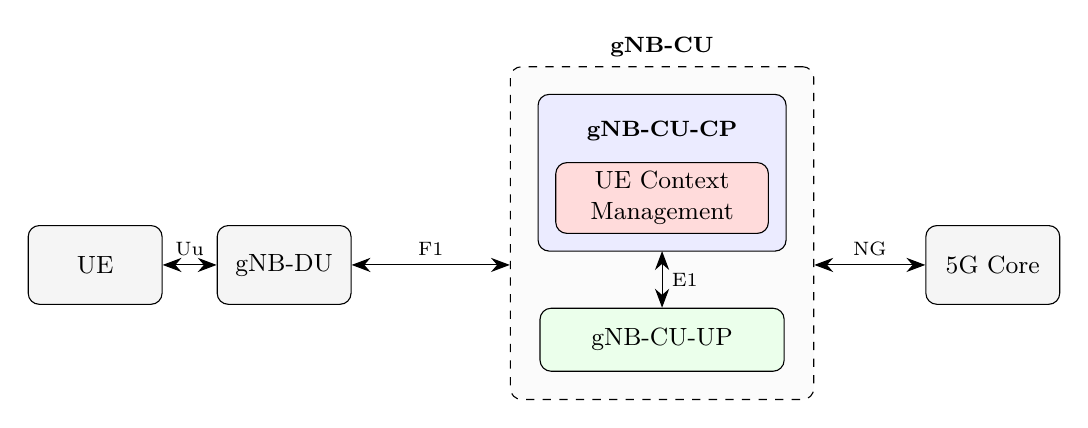
\begin{tikzpicture}[
    font=\small, >={Stealth[length=2.4mm]},
    box/.style={draw, rounded corners, minimum height=1.0cm, minimum width=1.7cm,
                align=center, fill=gray!8},
    cpbox/.style={draw, rounded corners, align=center, fill=blue!8},
    upbox/.style={draw, rounded corners, minimum width=3.1cm, minimum height=0.8cm,
                  align=center, fill=green!8},
    uecm/.style={draw, rounded corners, minimum width=2.7cm, minimum height=0.62cm,
                 fill=red!14, align=center}
  ]
  \node[box] (ue) at (0,0)   {UE};
  \node[box] (du) at (2.4,0) {gNB-DU};

  % Control plane, with UE Context Management shown nested inside it
  \node[font=\footnotesize\bfseries] (cpttl) at (7.2,1.7) {gNB-CU-CP};
  \node[uecm] (uecm) at (7.2,0.85) {UE Context\\ Management};
  % User plane
  \node[upbox] (up) at (7.2,-0.95) {gNB-CU-UP};

  % The background layer paints in source order and the central unit's fill is opaque, so
  % the control-plane box has to be drawn after it. Node (cp) carries the geometry that the
  % central unit and the E1 arrow are measured against.
  \begin{scope}[on background layer]
    \node[fit=(cpttl)(uecm), inner sep=6pt] (cp) {};
    \node[draw, dashed, rounded corners, fill=gray!3,
          fit=(cp)(up), inner sep=10pt, label={[font=\footnotesize\bfseries]above:gNB-CU}] (cu) {};
    \node[cpbox, fit=(cp), inner sep=0pt] {};
  \end{scope}

  \node[box] (core) at (11.4,0) {5G Core};

  \draw[<->] (ue) -- node[above,font=\scriptsize]{Uu} (du);
  \draw[<->] (du.east)         -- node[above,font=\scriptsize]{F1} (cu.west |- du);
  \draw[<->] (cu.east |- core) -- node[above,font=\scriptsize]{NG} (core.west);
  \draw[<->] (cp.south) -- node[right,font=\scriptsize]{E1} (up.north);
\end{tikzpicture}
\caption[Where the studied subsystem sits in the 5G NG-RAN]{Where the studied subsystem sits in the 5G NG-RAN. UE Context Management is
highlighted inside the gNB-CU-CP.\label{fig:ngran}}
\end{figure}

\section{Research gap}\label{sec:gap}
The RAN control plane has many threads and tight delay limits.
What sets the quality of the network is the slow tail under too much load, not the average throughput.
C++ gives the control and the speed this domain needs.
It also leaves whole families of memory bugs and thread bugs to be found after the program has been built.
Rust promises to block those families when the code is compiled, with no extra cost at run time.
It also offers a way to adopt it step by step, by calling Rust through the C application binary interface (ABI).
An ABI is the binary contract that lets one compiled program call another.

The domain is not unstudied.
The amount of earlier work is easy to miss, because almost none of it is in the usual paper indexes.
Five master's theses, all done at Ericsson and hosted by the vendor, have compared languages for RAN and telecom software.
One weighs run-time cost against how fast people can build, across C++, Rust, and Go~\cite{karlback2021ran}.
One asks whether Rust could replace C in RAN node management~\cite{olsson2023ranmgmt}.
One builds a packet processor in async Rust, with one thread per core, and measures it against the Data Plane Development Kit (DPDK) program it copies~\cite{olsson2023asyncpackets}.
DPDK is a library for moving packets very quickly.
One measures median and p99 delay for control-plane steps across five async frameworks~\cite{arvidsson2025async}.
The last builds matched C++ and Rust versions of an Abstract Syntax Notation One (ASN.1) decompiler and compares them with statistical tests~\cite{emberg2023asn1}.
ASN.1 is the notation used to describe the messages these protocols exchange.
All five are directly relevant. They do not all favour Rust.
Olsson and Stenstr\"om's packet processor reaches a fifth to a half of DPDK's throughput, with much worse latency~\cite{olsson2023asyncpackets}.
Arvidsson and Kaller's Rust p99 rises more steeply once the rate passes a threshold~\cite{arvidsson2025async}.
Karlb\"ack and Or\"o pick C++ where speed is critical. They still find Rust lightest on peak memory~\cite{karlback2021ran}.
Olsson's management software is as fast as C, or faster, and it uses more peak memory~\cite{olsson2023ranmgmt}.
Emberg and Wadsten's pair is comparable in one session and $85$--$91\%$ worse in the next~\cite{emberg2023asn1}.

Three of those studies change the language together with the run-time and the thread model.
A measured gap then cannot be blamed on the language alone. It may come from the framework~\cite{karlback2021ran,olsson2023asyncpackets,arvidsson2025async}.
In the packet-processor study the DPDK program does two to five times as much work~\cite{olsson2023asyncpackets}.
A compiler does not move throughput that far. The run-time does.
Olsson's management study and Emberg and Wadsten do not change the run-time when they change the language~\cite{olsson2023ranmgmt,emberg2023asn1}.
They report run time and peak memory, not the slow tail under rising load.
Emberg and Wadsten come closest in method to this thesis.
They still measure a stateless transform, a conversion that does not remember anything between calls.
It is not a stateful part with many threads.
Figure~\ref{fig:gapmap} places the five vendor theses beside the general-purpose comparisons~\cite{pereira2017energy} and the matched systems-software pairs~\cite{emmerich2019drivers,suchert2023stamp}.
Each group holds some of what a fair test would need. None holds all of it.

That concentration is itself part of the gap.
All five studies come from one vendor.
Their conclusions have never been tested against another firm's software, targets, or house rules.
So what is known about this question is what one firm's frameworks say about it.
The published record on the other side is thinner.
There is no study of Rust among the indexed papers of the vendor hosting this work.
The nearest peer-reviewed stance from that side argues for making memory-error checking practical at run time.
It does not argue for replacing that checking with a guarantee at compile time~\cite{gjomemo2016mesc}.
That run-time strategy is the one this thesis tests against.

\begin{figure}[ht]
\centering
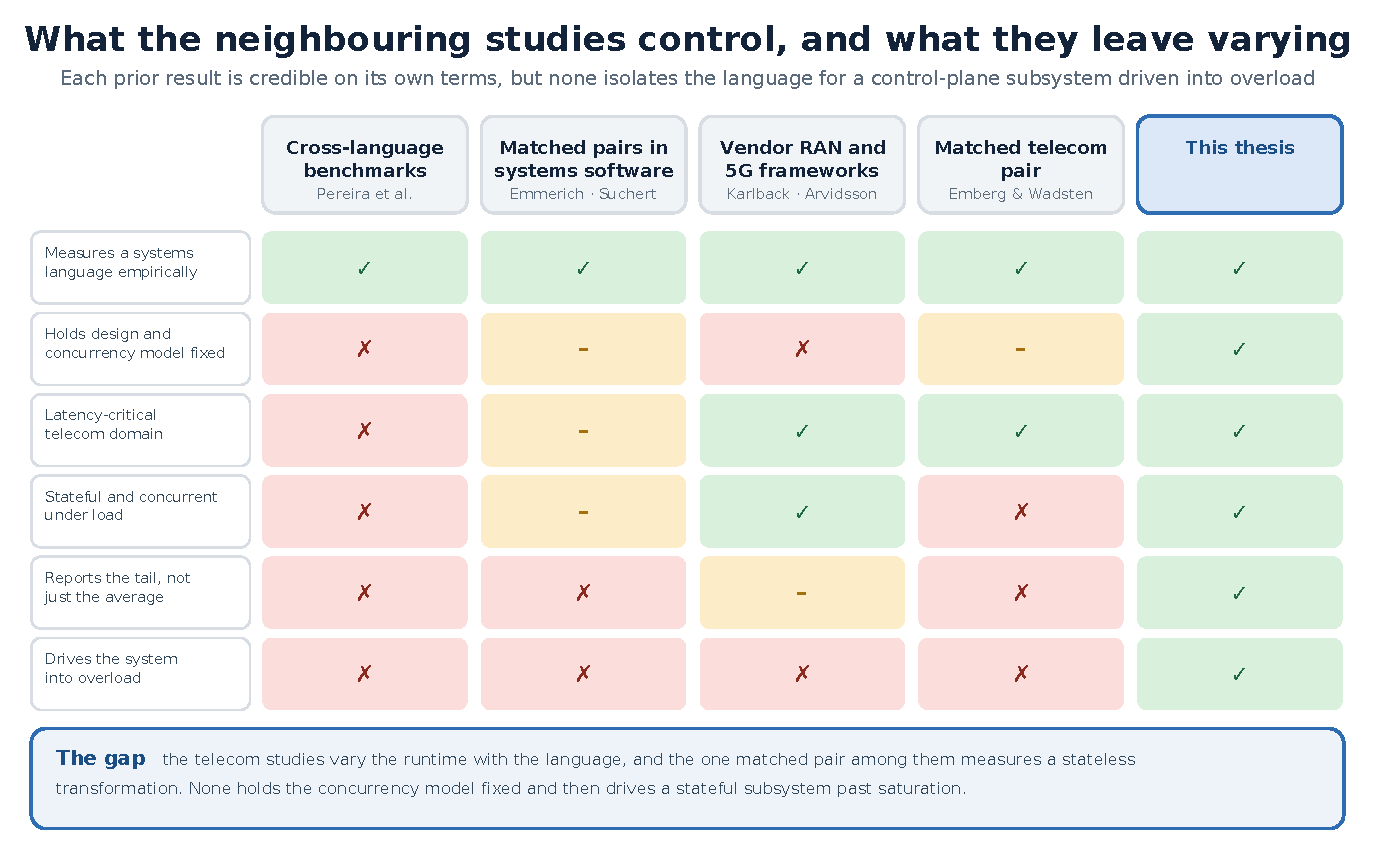
\includegraphics[width=\linewidth]{diagrams/pdf/29_research_gap.pdf}
\caption[What the neighbouring studies control, and what they leave varying]{What the neighbouring studies control, and what they leave varying. Each row is a
property a controlled answer would need, and each column is a group of studies.
The vendor-RAN column is the Ericsson theses other than Emberg and Wadsten,
who have their own column because they hold the design closer.\label{fig:gapmap}}
\end{figure}
% The last paragraph of the section runs one line onto the next folio
% once the figure is at full text width. A modest enlarge keeps that
% line with the figure instead of leaving it alone in front of Chapter 3.
\enlargethispage{96pt}

What is missing is a direct, controlled test of a typical control-plane part.
The open questions are these.
Does Rust hold its tail delay under too much load against modern C++, when the thread model, the operations, and the data layout stay fixed?
Which bug types does it remove, and at what stage are the rest caught?
What does its safety model cost in throughput, CPU, and memory?
What does step-by-step adoption cost in practice?
Closing this gap is the purpose of the four research questions.
The next chapter grounds them in the part under study, the bug types, and the timing at stake.
It also sets out the method.


\chapter{Research Methodology\label{chapter:methodology}}
\chaptermark{Methodology}

The last chapter set out the gap. This chapter says how the study closes it.

\section{The UE Context Management subsystem}\label{sec:uecm}
The part under study is a UE Context Management service.
Its operations follow the life of a UE context, the execution of RRC procedures~\cite{3gpp38331}, and the mobility and handover work that the 3GPP design assigns to the control-plane part of a split gNB (Section~\ref{sec:ranarch}).
Figure~\ref{fig:fsm} shows that life cycle. Both versions encode it the same way.
The mixed workload of Section~\ref{sec:workload} walks each UE through that machine.

A context starts Idle. A setup moves it to Connected. From Connected it can be reconfigured and then return, or it can be released. A release from Idle is also allowed. Signalling and adding a data radio bearer stay in Connected. An operation that is illegal in the current state returns an error and does not change the state.

\begin{figure}[ht]
\centering
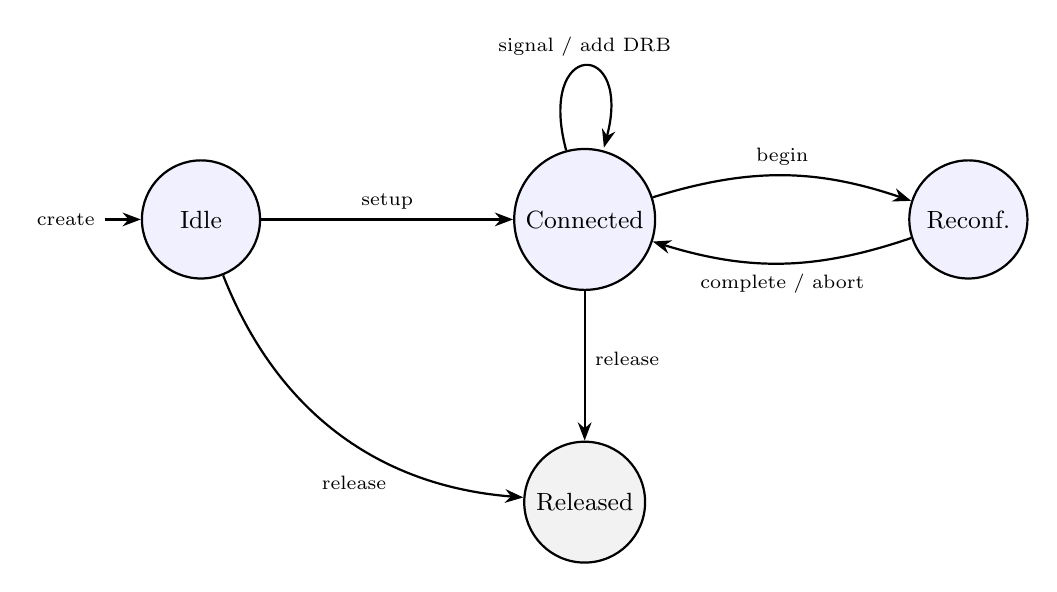
\begin{tikzpicture}[
    ->, >=Stealth, node distance=3.2cm, font=\small,
    every state/.style={draw, minimum size=1.5cm, fill=blue!6, thick},
    every edge/.style={draw, thick}
  ]
  \node[state, initial, initial text=\scriptsize create] (idle) {Idle};
  \node[state, right=of idle] (conn) {Connected};
  \node[state, right=of conn] (reconf) {Reconf.};
  \node[state, below=1.9cm of conn, fill=gray!10] (rel) {Released};

  \path (idle)  edge node[above,font=\scriptsize]{setup} (conn)
        (conn)  edge[bend left=18] node[above,font=\scriptsize]{begin} (reconf)
        (reconf) edge[bend left=18] node[below,font=\scriptsize]{complete / abort} (conn)
        (conn)  edge node[right,font=\scriptsize,pos=0.45]{release} (rel)
        (idle)  edge[bend right=32] node[below=8pt,font=\scriptsize,pos=0.55]{release} (rel);
  \path (conn) edge[loop above] node[font=\scriptsize]{signal / add DRB} (conn);
\end{tikzpicture}
\caption[UE-context lifecycle state machine]{UE-context lifecycle state machine.
Operations invalid for the current state return an error instead of changing
state.\label{fig:fsm}}
\end{figure}

UECM is core RAN layer-3 work. Layer 3 is the signalling layer above the radio itself.
It has the traits that make live control-plane code hard.
Each UE has state that changes. The order of operations is strict. Many UEs run at once.
The delay targets are the ones the 5G system sets for control-plane procedures~\cite{3gpp38913,3gpp22261}.
Findings about how a language handles those traits apply most directly to other stateful, multi-thread control-plane services of this kind.
The part is also small enough to specify in full and build twice.
That is what makes a comparison with matching tests possible.

The interface is small and follows the life cycle.
It can create and release a context, set up a connection, handle a signalling message during the session, add a data radio bearer, begin, complete, or abort a reconfiguration, and look up a context's state under load.
Each operation is defined for each state of Figure~\ref{fig:fsm}.
An illegal operation returns a typed error and leaves the context unchanged.
That closed set lets the same tests and the same workload drive both versions along the same paths.

RQ2 needs a fixed catalogue of bugs, not a loose list of hazards.
One is built from this operation set: $\FaultClasses$ types, in two groups of seven.
Seven come from inside the region that safe Rust claims to govern.
Seven were chosen because safe Rust is expected not to prevent them.
Each expectation was written down before the programs were run.
Section~\ref{sec:safetyresults} reports what each one did.

The tail is the metric for two reasons.
First, one action the user sees, such as a call setup or a handover, becomes many control-plane operations that depend on each other.
The slowest one decides when the action is finished.
A busy site drives thousands of such procedures per second, so a far-tail point is reached often enough to matter.
Second, the shape of failure matters.
Under an open-loop clock the sender keeps to its schedule and does not wait for replies.
The achieved rate can then track the offered load until either the service, or work inside the timed sender, becomes the limit.
Delay then rises sharply.
That is why this study sweeps past the apparent saturation point, the load where the service stops keeping up, and checks what the timed path actually contains.

\section{Research approach}\label{sec:approach}
The study runs experiments. It also builds the thing it measures: a matched pair of versions, plus the harness that drives them.
Both are built from one frozen specification.
Evidence comes from three separate methods.
A load sweep, which raises the offered rate step by step, contributes to RQ1 and RQ3.
Controlled fault injection, which plants known bugs on purpose, answers RQ2.
An FFI migration prototype answers RQ4.
A weakness in one method does not carry into the other claims.
For example, the host machine can move the tail. That does not change what the fault-injection result says.

Each question asks how one outcome depends on one variable, the language.
The language has to be the only planned difference between the two programs under test.
That rules out the most common way to compare languages.
In that form, two programs written separately are measured, and the gap is taken to be the language.
Such a gap also carries the design, the libraries, and the skill of the authors.
Building both sides from one specification removes that confound.
Where a question can be answered with numbers, it uses numbers.
Where it cannot, the answer still follows a fixed plan, in words.
That is how this study treats the kind of guarantee in RQ2.
RQ4 asks about the design cost of the application programming interface (API), the set of calls the rest of the system is allowed to make.

The closest earlier work is the five vendor-hosted theses of Section~\ref{sec:gap}.
They appear in no citation database. They had to be found by searching each university's own archive by hand.
The same searches found no Finnish thesis on Rust in a radio-access setting.
They found no indexed paper mentioning Rust from the vendor hosting this work.
The search returned no study that measures the tail of a Rust version and a C++ version of the same stateful, multi-thread control-plane part under too much load.

Table~\ref{tab:design} maps each research question to the method, the artefact, the data, and the metric that answer it.
RQ1 and RQ3 share H1.
H1 was worded to cover a speed tie both in delay and in resource use.
That wording turns out to be the hypothesis's main weakness, because those are not one quantity.
RQ2 does not depend on the host machine.
RQ4 depends on the host along one axis.
Build time is a timing, so it is read as a ratio between two toolchains measured in turn on one machine.

\begin{table}[ht]
\centering
\small
\caption[How each research question is answered]{How each research question is
answered. RQ1 and RQ3 carry two methods rather than one. Below saturation the
sweep measures the round-trip a deployment would experience. The split of the
core from the handoff measures the part the language can own, while later
diagnostics test whether high-load recorder work contaminates the sweep.
\label{tab:design}}
\renewcommand{\arraystretch}{1.2}
\setlength{\tabcolsep}{4pt}
\begin{tabular}{@{}p{0.07\linewidth} p{0.27\linewidth} p{0.27\linewidth} p{0.27\linewidth}@{}}
\hline\hline
RQ & Method & Artefact / data & Primary metric \\
\hline
RQ1 & Load sweep to overload, interleaved repeats & Benchmark harness, latency histograms &
median, p99/p99.9/p99.99, and maximum vs.\ offered load \\
RQ3 & Same sweep, resource capture & \texttt{getrusage} samples per run &
peak resident set size (RSS), CPU, throughput \\
RQ1, RQ3 & Core called directly, then through the service &
Matched microbenchmark pair &
operation vs.\ cross-thread handoff \\
RQ2 & Controlled fault injection & Defect catalogue, three C++ sanitisers,
\texttt{rustc}, Loom/Shuttle, Miri &
compile-time / runtime / undetected \\
RQ4 & FFI migration prototype & C++ host $+$ Rust C-ABI boundary &
boundary size, \texttt{unsafe} scope, per-call cost \\
\hline
\end{tabular}
\end{table}

\section[Methods per research question]{Methods per research question, in outline}\label{sec:methodbrief}
RQ1 and RQ3 use an open-loop load sweep, from light load to well past saturation.
Open-loop means the generator keeps to its send schedule instead of waiting for replies~\cite{schroeder2006openclosed}.
The four build variants take turns inside each repeat, so none of them always runs first.
A variant here is one combination of language and memory allocator.
A second timing splits the core operation from the cross-thread handoff around it.
The end-to-end round trip bundles two costs of two kinds. Only one of them can differ between the languages.
A third timing takes the contended queue and the reply handle on their own.
Later full-grid diagnostics move or remove the histogram fill from the timed sender path.
The histogram fill is extra bookkeeping that records how late a call was.
Together these tests narrow the overload explanation.
The comparison across setups does not isolate one cause.

RQ2 is answered by controlled fault injection~\cite{natella2016fault}.
Each bug type is a small program of its own, written in both languages.
The C++ side is built and run under AddressSanitizer, ThreadSanitizer, and UndefinedBehaviorSanitizer.
A sanitiser is a checking tool that watches the running program for one family of bugs.
The safe-Rust side is compiled and, where it compiles, run under a bounded timeout.
No static analyser is run, on purpose.
The C++ columns then report the tooling this study ran.
They do not report a ceiling on what C++ tooling could find.
RQ4 is answered by a working prototype in the direction a real migration takes.
A C++ host calls an unchanged Rust core across a C ABI.
This boundary is called the FFI seam here.
It is the thin layer that converts between the C++ host and the Rust core.
The per-call cost is measured on a real operation. It is not inferred from an empty crossing.
Memory bugs that cross a language sit at that seam~\cite{li2022crosslang}.

\section{Fairness as a controlled variable}\label{sec:controlsbrief}
A language comparison is only as good as the things it holds fixed.
The specification is frozen before either version exists.
The thread model, the allocator and its arena count, the optimisation level, the hash function, the histogram method, and the load schedule match across the two sides.
They are never tuned per side.
Where the two languages could not be written alike, the gap is logged instead of quietly resolved.
The two sides are shown to match by comparing logs operation by operation.
For a given seed they also run the same operations in the same order.
The four variants take turns on the same pinned cores inside each repeat.
That keeps recent cache contents and recent branch guesses close, because the same work runs one after another.
The test does not empty the cache between variants.
It also does not first train the CPU on those branches.
It holds the work and the cores fixed.
It does not hold the CPU's recent memory and branch history fixed.

\section{Statistical treatment}\label{sec:statsbrief}
The statistical design was fixed in advance.
The family of comparisons to be tested was listed before the campaign ran.
A load picked after seeing the results cannot join that family.
Each comparison is an exact paired permutation test over \NRepeats{} interleaved repeats, with a bootstrap confidence interval~\cite{efron1993bootstrap}, and Holm correction across the family~\cite{holm1979simple}.
In plain terms, the two languages are compared on the same repeats, the test asks how often a gap that large would appear by chance, and the Holm step stops a long list of tests from inventing a false hit.
The floors the test can reach ($\MinAttainableP$ uncorrected, $\CorrectedFloor$ corrected) are quoted so that a reported null can be told apart from a mathematical limit of the test.
Throughput at the representative load is reported but not tested, because it is pinned to the offered rate. If the service keeps up, throughput equals the rate that was sent.
Jitter, the small wobble from call to call, is outside the research questions.
The maximum is too sensitive to one disturbed operation for pairing to rescue it.
The pooled p99.99 far tail uses the operation as its unit, so it has no interval across repeats to test.
No latency percentile is tested after saturation.
Past that point, the sender's schedule drifts, and the recorded percentile becomes a lower bound rather than an estimate of how long the service itself took.

\section{Reproducibility and research artefacts}\label{sec:repro}
A third party can rebuild the results without access to Nokia's private code.
The versions are driven entirely by the public frozen specification.
The benchmarking harness, the fault catalogue and its runner, and the FFI prototype are published with the thesis.
Each plot of measured data is rebuilt by one script from the raw logs.
So is each quoted number in the results.
The script is \texttt{bench/refresh\_thesis.sh}.
That claim does not cover the hand-drawn diagrams, which explain a concept rather than report a result.
Running the same scripts over another host's campaign rebuilds the artefacts by the same procedure. It does not reproduce the same values.

The logs that the script reads are part of the package.
Each campaign has its own script and its own macro prefix, so a figure from one campaign cannot leak into a sentence about another.
Each run's host setup is recorded and stored beside the campaign data.
Nothing in the results chapters is typed from those files by hand.

\chapter{Design and Implementation\label{chapter:design}}
\chaptermark{Design}

Nothing is built until the specification is frozen.
It fixes the public API, the UE state machine, the data layout and the steps on it, the locks and the shard size, and the thread model.
Both versions follow it.
The test then times the language, not a gap of design or of skill.
The specification is itself an output of the study.
It is the main control against the bias of the person who wrote both versions.

One thread model is used on both sides: shared-nothing, with one thread per shard.
Shared-nothing means the workers do not share the UE records.
A shard is one slice of the identifier space, owned by one thread.
That layout is known to change tail delay by itself~\cite{enberg2019threadpercore}.
The layout is held fixed so the comparison stays fair.
A production gNB-CU-CP schedules UE work differently.
The identifier space is split into shards.
Each shard is owned by one worker thread.
That thread alone reads or changes it, so no lock guards context state.
Callers send a request to the owning shard's bounded queue and wait on a one-shot reply handle.
The queue blocks when it is full. That is on purpose.
A rule that dropped requests would hide overload.
This study needs overload to show up as delay.
The only shared mutable state either version allows is one atomic counter.
No control flow depends on its value.
Figure~\ref{fig:arch} shows the data flow.
There is one multi-producer, single-consumer (MPSC) queue per shard.
Many senders can write to it. Only the shard's worker reads it.
The worker drains it first in, first out (FIFO).

\begin{figure}[ht]
\centering
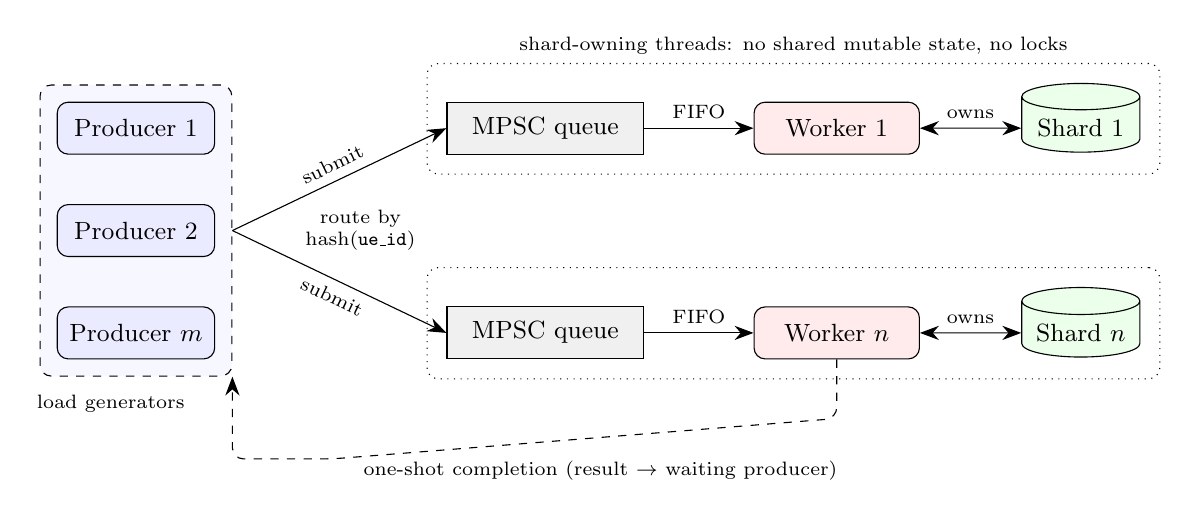
\begin{tikzpicture}[
    font=\small,
    prod/.style={draw, rounded corners, minimum width=2.0cm, minimum height=0.66cm, fill=blue!8},
    queue/.style={draw, minimum width=2.5cm, minimum height=0.66cm, fill=gray!12},
    worker/.style={draw, rounded corners, minimum width=2.1cm, minimum height=0.66cm, fill=red!8},
    store/.style={draw, cylinder, shape border rotate=90, aspect=0.25, minimum width=1.5cm, minimum height=0.85cm, fill=green!8},
    lane/.style={draw, dotted, rounded corners, inner sep=7pt},
    >={Stealth[length=2.4mm]}
  ]
  \node[prod] (p1) at (0,1.3)  {Producer 1};
  \node[prod] (p2) at (0,0.0)  {Producer 2};
  \node[prod] (p3) at (0,-1.3) {Producer $m$};
  \begin{scope}[on background layer]
    \node[draw, dashed, rounded corners, fill=blue!3, fit=(p1)(p2)(p3), inner sep=6pt] (pg) {};
  \end{scope}
  \node[font=\scriptsize, anchor=north] at ([xshift=-0.32cm,yshift=-3pt]pg.south) {load generators};

  \node[queue] (q1) at (5.2,1.3)   {MPSC queue};
  \node[worker](w1) at (8.9,1.3)   {Worker 1};
  \node[store] (s1) at (12.0,1.3)  {Shard 1};
  \node[queue] (qn) at (5.2,-1.3)  {MPSC queue};
  \node[worker](wn) at (8.9,-1.3)  {Worker $n$};
  \node[store] (sn) at (12.0,-1.3) {Shard $n$};
  \begin{scope}[on background layer]
    \node[lane, fit=(q1)(s1)] (lane1) {};
    \node[lane, fit=(qn)(sn)] (lanen) {};
  \end{scope}
  \node[font=\scriptsize] at (8.35,2.35) {shard-owning threads: no shared mutable state, no locks};

  \node[font=\scriptsize, align=center, fill=white, inner sep=2pt] at (2.85,0) {route by\\ hash(\texttt{ue\_id})};
  \draw[->] (pg.east) -- (q1.west) node[midway, above, sloped, font=\scriptsize]{submit};
  \draw[->] (pg.east) -- (qn.west) node[midway, below, sloped, font=\scriptsize]{submit};

  \draw[->]  (q1) -- node[above, font=\scriptsize]{FIFO} (w1);
  \draw[->]  (qn) -- node[above, font=\scriptsize]{FIFO} (wn);
  \draw[<->] (w1) -- node[above, font=\scriptsize]{owns} (s1);
  \draw[<->] (wn) -- node[above, font=\scriptsize]{owns} (sn);

  \draw[->, dashed, rounded corners=4pt]
      (wn.south) -- ++(0,-0.75) -- (2.5,-2.9) -| (pg.south east);
  \node[font=\scriptsize] at (5.9,-3.05) {one-shot completion (result $\rightarrow$ waiting producer)};
\end{tikzpicture}
\caption[Shared-nothing, thread-per-shard architecture]{Shared-nothing,
thread-per-shard architecture. Producers submit to a bounded MPSC queue per
shard, and that shard's worker drains it.\label{fig:arch}}
\end{figure}

Fairness is kept below the design as well as in it.
Both builds link the same \texttt{jemalloc}, which is a replacement memory allocator.
Both also keep a build that uses the system's own allocator, as a control.
Both compile at the same optimisation level.
Both record delay through one high-dynamic-range (HDR) histogram, set up the same way~\cite{tene_hdrhistogram}.
An HDR histogram can record both very short and very long delays without losing the slow tail.
Hashing is pinned on both sides.
SplitMix64 assigns the shard~\cite{steele2014splitmix}.
FNV-1a, the Fowler--Noll--Vo hash~\cite{rfc9923}, is used inside the map.
C++'s default hash of an integer is often just the number itself.
Rust's default hash is deliberately stronger.
Left as they came, the two standard libraries would have been part of the measurement.

Where the languages cannot meet a need the same way, the gap is written into a forced-idiom log and then measured.
Two of those gaps were candidates for the overload result of Section~\ref{sec:overload}, the result read from the campaign clock.
One is the bounded queue.
Rust takes it from \texttt{sync\_channel}.
C++23 still has no such primitive, so C++ builds one from a mutex and two condition variables.
The other is the reply handle: \texttt{std::promise} on the C++ side, against a fresh \texttt{mpsc} channel per request on the Rust side.
Tests of those primitives, and a replacement reply handle, do not reproduce the two large campaign gaps.
A third gap carries the core-operation result of Section~\ref{sec:perfresults}.
The per-shard container is each language's own standard hash map.
A fourth is the request encoding.
C++ has no payload-carrying enumeration in this idiom, so a request becomes a tagged struct that holds every field any operation might need.
That struct is $\CppRequestBytes$~bytes, against Rust's $\RustRequestBytes$.
The net result is a Rust core $\NlocRise\%$ longer in lines of code.
Its branching complexity is $\CcnTotalDrop\%$ lower~\cite{lizard}.
The Rust library contains no \texttt{unsafe} at all.
\texttt{unsafe} is the Rust keyword that switches the compile-time checks off for a marked region.

Parity is tested. It is not assumed.
Language-neutral test vectors run in both versions, and their logs are compared operation by operation.
A comparison of the two logs cannot tell ``both correct'' from ``both wrong in the same way''.
A third version, in Python, acts as an independent oracle.
It has to reproduce all $\ConfHandOps$ hand-derived expectations before it may generate any of its own.
A campaign of $\ConfGenOps$ generated operations found no mismatch.
The C++ side runs under AddressSanitizer, ThreadSanitizer, and UndefinedBehaviorSanitizer.
The Rust side runs under Miri, an interpreter that checks Rust's safety rules as the program runs.
A clean sanitiser result only covers the code that actually ran.

\chapter{Experimental Setup and Evaluation\label{chapter:eval}}
\chaptermark{Evaluation}

This chapter starts with the test machines and the work they run. The results then follow by load, and then by the rest of the questions.

\section{Testbed setup\label{sec:testbed}}
Some numbers in this chapter come from the tools and the code.
Other numbers depend on the machine they ran on.
The reported campaign comes from one bare-metal host, a machine with no virtual machine in the way, a single-socket \MainCpu{}.
Each core runs one thread. Extra threads on a core are \MainSmt{}.
The host runs \MainHostDistro{} on kernel \MainKernel{}.
Linux can raise and lower each core's clock as load and heat change.
The clock is held fixed. The governor is \MainGovernor{}, and boost is off.
The test may use only cores \MainPinned{}. There is no hypervisor.
The program runs on the host itself, not inside a virtual machine.
On those cores the kernel turns off its timer tick (\texttt{nohz\_full}).
If left on, those ticks would show up in the delay numbers.
The study does not use \texttt{isolcpus}.
That flag also stops the kernel from sharing work across the allowed cores.
Each test thread then lands on one core.

The build tools are not the ones installed on the host.
Both sides are built and run inside an image that carries \MainDistro{} with \texttt{g++~\MainGpp} and \texttt{rustc~\MainRustc}.
The image pins the \texttt{gcc-toolset} major version, not the point release.
The earlier sweep on a virtual machine then built with \texttt{g++~\GuestGpp}, one GNU Compiler Collection (GCC)~15 release earlier.
An image still uses the kernel of the host it sits on.
The two sweeps then differ in the hardware, in the kernel (\MainKernel{} against \GuestKernel{}), and in that compiler release.

Until late in the work the sweep ran on a Kernel-based Virtual Machine (KVM) on an \GuestCpu{}, with none of the core controls above.
The capture records the hypervisor as \GuestVirt{}, the guest userland as \GuestDistro{}, and the guest kernel as \GuestKernel{}.
On that host the $95\%$ band on one variant's p99 spans $\GuestPNineNineMaxCI\,\mu$s.
The four variants' p99 values differ by $\GuestPNineNineRange\,\mu$s.
The noise on one variant was larger than the gap between all four.
That sweep is kept. It uses the same design as this one.
The two can then be set next to each other to ask which findings belong to the code.
A third sweep, on a second bare-metal \BmCpu{}, uses a new shard count, load grid, run count, and tools.
It tests whether the findings hold when those things change together, not any one of them on its own.

\section[Workload and measurements]{Workload and measurements\label{sec:workload}}
The work is made for the test. The steps it takes come from the 3GPP rules~\cite{3gpp38401,3gpp38331}.
A driver that always sends the same steps walks each UE through the connection life cycle those rules define.
The \emph{signal} workload first connects a set of UEs, then sends the same signal call again and again.
That picks out the common path.
The \emph{mixed} workload walks each UE through context creation, setup, signal, bearer setup, reconfiguration or handover, and release.
A fixed random order makes both sides see the same counts of each call kind for a given seed.
That is also a check that the two sides did the same work.
Figure~\ref{fig:workload} shows the two loads and the steps the mixed one walks.

\begin{figure}[ht]
\centering
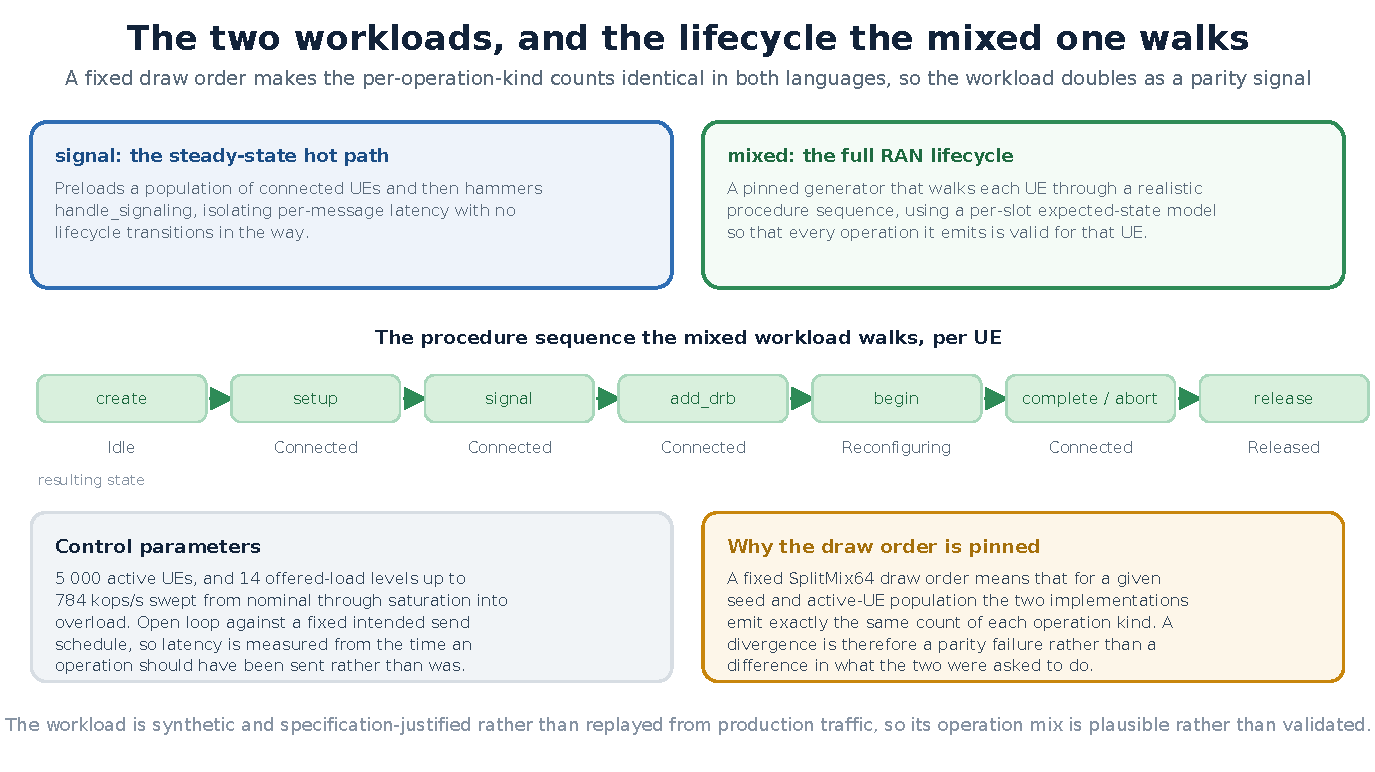
\includegraphics[width=0.78\linewidth]{diagrams/pdf/27_workload_timeline.pdf}
\caption[The two workloads, and the lifecycle the mixed one walks]{The two
workloads, and the lifecycle the mixed one walks. Signal repeats the common
path, and mixed walks each UE through the procedure sequence drawn
below.\label{fig:workload}}
\end{figure}

The steps match the 3GPP rules. Those rules do not set the mix of call types.
A real cell's handover rate depends on the site and the time of day, and no public figure fixes it.
A mix that does not match a real cell moves both sides by the same amount.
It limits how far the numbers travel to a real network. It does not make the test unfair.
The sender keeps to its plan even if the service is late. That is the open-loop rule.
The histogram is corrected so a stall does not hide missing replies.
That correction is for coordinated-omission bias.
If the recorder only times the calls that finished, it misses the ones that were stuck~\cite{schroeder2006openclosed,tene_hdrhistogram}.
Each load is run \NRepeats{} times.
The four language and heap variants take turns inside each run.
Each point is a median with a bootstrap $95\%$ band~\cite{georges2007rigorous,efron1993bootstrap}.
The band is the range in which the median would be expected to fall if the experiment were repeated.

The load used for the resource plots is $\ReprLoad$~kilo-operations per second (kops/s).
It is a chosen value, not one derived from the sweep.
The first rule this study used was the peak load whose p99 stayed under $5$~ms.
On the virtual machine that rule landed on the noise of the host.
On a quiet host it climbs until the service can no longer keep up.
It is kept only as a check.
The lowest finished rate among the four variants is $\SatKnee$~kops/s, reached when the sent load is $\TrackingLoad$~kops/s.
That finished rate is the knee: the point where raising the offered load no longer raises the rate the service completes.

\section{Results}
The safe-code results, and most of the migration results, do not depend on which host was used.
The speed and memory results do.
Each figure below was timed on the host of Section~\ref{sec:testbed} unless the caption says so.

\subsection{Below saturation (RQ1, RQ3)}\label{sec:perfresults}
Saturation here means the service can no longer finish work as fast as it is offered.
At the representative load of $\ReprLoad$~kops/s, every variant still keeps up with the sent load.
The four variants' medians lie within $\PFiftyRange\,\mu$s of each other, a spread of $\PFiftySpread\%$.
A paired test still finds a gap of $\PFiftyDiffAbsMax\,\mu$s in Rust's favour, under both heaps.
Figure~\ref{fig:loadsweep} shows the sweep behind that number.
The higher tails can now be read as well.
The widest band on one variant's own p99 spans $\PNineNineMaxCI\,\mu$s.
The four variants' p99 values differ by $\PNineNineRange\,\mu$s.
So the noise on one variant is smaller than the gap between them.
On the virtual machine the same two sizes were $\GuestPNineNineMaxCI\,\mu$s against $\GuestPNineNineRange\,\mu$s, the other way around.
Both p99 rows and both p99.9 rows clear the Holm correction, \NTailSignificant{} rows in all, in the same direction as the median.
Table~\ref{tab:latency} reports p99.9 and the maximum at the chosen load.
The maximum is kept out of the tested family, as the pooled p99.99 is.

\begin{table}[ht]
\centering
\small
\caption[Per-operation latency at the representative load]{Per-operation latency,
in microseconds, at $\ReprLoad$~kops/s. The median over \NRepeats{} repeats sits
above its bootstrap $95\%$ interval. $^{\dagger}$The p99.99 column is pooled across
repeats, so it has no interval. The maximum has a repeat-wise interval but stays
outside the tested family because one disturbed operation can determine it.
\label{tab:latency}}
\LatencyTabular
\hline\hline
\LatencyHead \\
\hline
C++ (system alloc) & \mci{217.2}{163.8}{237.2} & \mci{355.1}{289.3}{389.4} & \mci{674.3}{395.3}{1538.0} & \mci{2170}{910}{5594} \\
C++ (jemalloc) & \mci{225.8}{181.1}{261.2} & \mci{410.1}{305.7}{11280.4} & \mci{1188}{544}{14213} & \mci{3590}{1472}{16291} \\
Rust (system alloc) & \mci{214.3}{191.6}{238.8} & \mci{376.3}{330.2}{3629.1} & \mci{1068}{504}{6955} & \mci{2404}{1129}{9667} \\
Rust (jemalloc) & \mci{208.4}{193.7}{223.1} & \mci{388.9}{342.3}{478.0} & \mci{763.4}{479.5}{4272.1} & \mci{2804}{1114}{7606}
\\
\hline
\end{tabular}
\end{table}

\begin{figure}[ht]
\centering
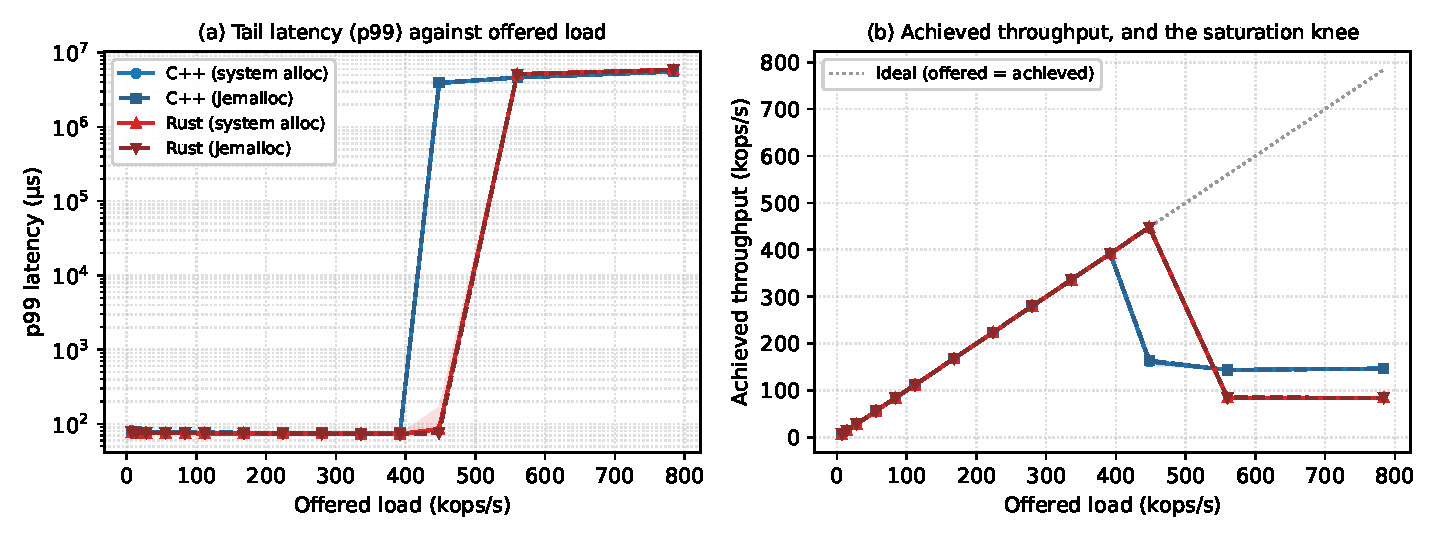
\includegraphics[width=0.78\linewidth]{figures/fig_load_sweep.pdf}
\caption[The load sweep: tail latency and achieved throughput]{The load sweep,
both panels against offered load. Lines are medians over \NRepeats{} repeats,
and the bands are bootstrap $95\%$ confidence intervals.\label{fig:loadsweep}}
\end{figure}

The far tail can be read here too.
The runs' histograms are pooled, which gives \FarTailSamplesMin{} to \FarTailSamplesMax{} calls per variant.
Pooling means the calls from every repeat are put into one histogram, so the very slow end has enough samples to see.
The two \FarTailLower{} variants sit below both C++ variants.
The widest pair differs by $\FarTailRange\,\mu$s.
The slowest Rust variant still sits $\FarTailLangSep\,\mu$s below the fastest C++ one.
Below here means faster: a smaller delay.
A second bare-metal host, at another shard count, agrees.
It runs $\BmFarTailCppLo$--$\BmFarTailCppHi\,\mu$s for the C++ variants against $\BmFarTailRustLo$--$\BmFarTailRustHi\,\mu$s for the Rust ones, and the ranges do not meet.
A second limit does not come from the host. No host would remove it.
An end-to-end round trip spends only $\BudgetCoreShareMax\%$ of its time on the work the language does.
The rest is passing the request to another thread, and that time is charged to the operating system.
When the work inside the language is this small, the time spent crossing from thread to thread dominates~\cite{zhou2025oltp}.
Figure~\ref{fig:e2eclock} draws that split.
This sweep cannot bound a language effect either way.
Figure~\ref{fig:budget} sets that limit beside what the sweep can still show.
Timed on its own, the core call is $\BudgetCoreRatio\times$ faster in \BudgetCoreFaster{}.
The test does not trace the cause.
The stock hash map is one candidate. The compiler's code generation may also own part of the gap.

\begin{figure}[ht]
\centering
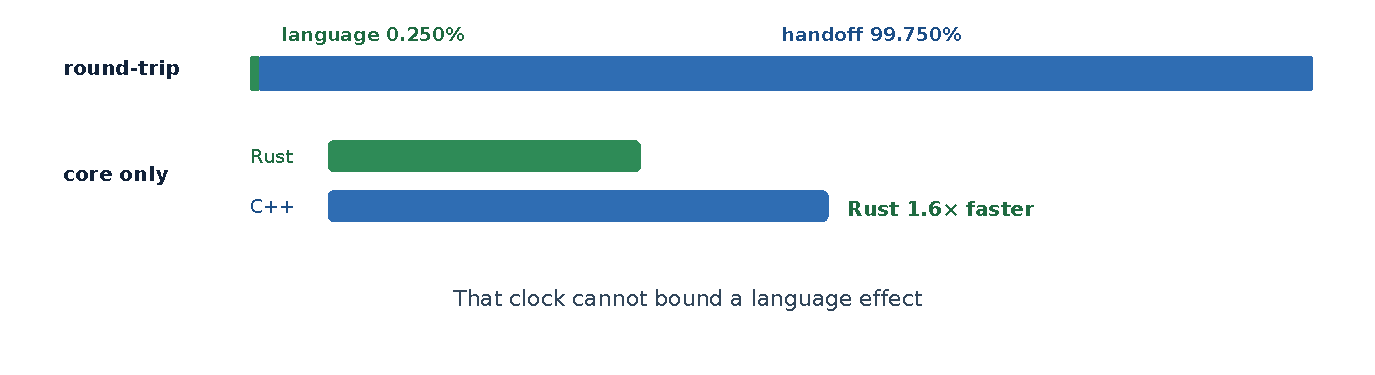
\includegraphics[width=0.78\linewidth]{diagrams/pdf/31_e2e_clock.pdf}
\caption[Where the end-to-end clock goes]{Where an end-to-end
round-trip's clock goes. The language share is
$\BudgetCoreShareMax\%$. A clock that spends the rest on handoff cannot bound
a language effect.\label{fig:e2eclock}}
\end{figure}

\begin{figure}[ht]
\centering
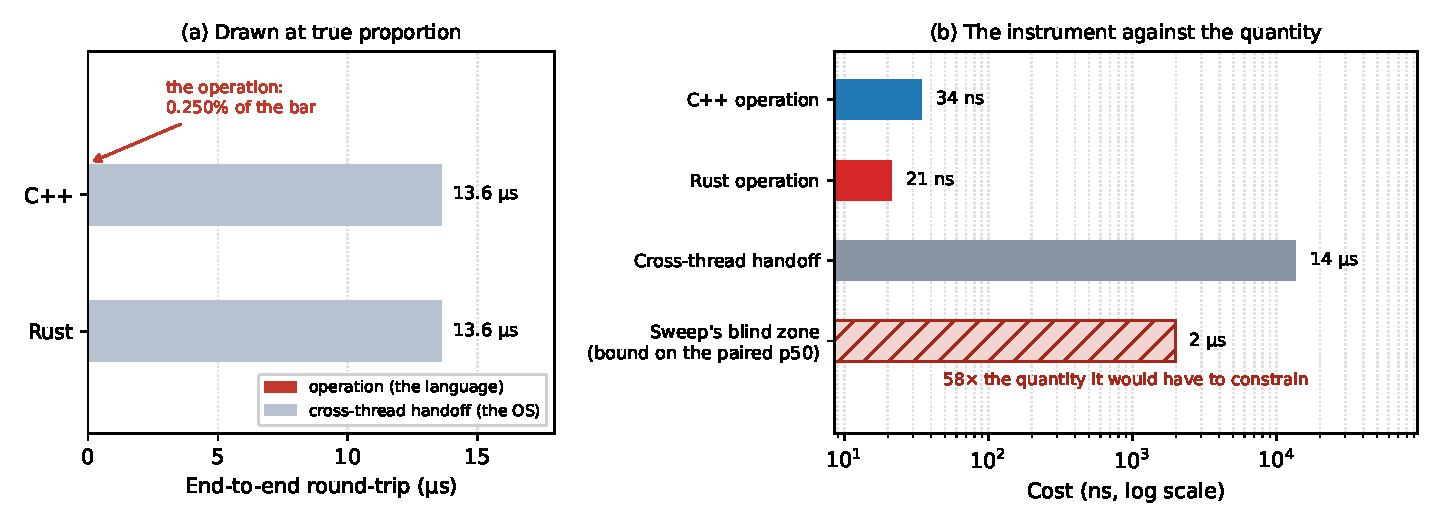
\includegraphics[width=0.78\linewidth]{figures/fig_budget.pdf}
\caption[The end-to-end operation decomposed, against what the sweep can resolve]{Where
an end-to-end round-trip's cost goes. \textbf{(a)} The round-trip at true
proportion. \textbf{(b)} Both operation measurements sit inside the sweep's
blind zone by a factor of $\BudgetBoundVsCore$.\label{fig:budget}}
\end{figure}

\subsection{Past saturation (RQ1)}\label{sec:overload}
The campaign clock is the timer used in the main experiment. It includes the service and the recorder that writes the histogram.
Under that clock, the four variants appear to stop keeping up at loads that do not match.
The Rust versions hold to $\TrackingLoadRust$~kops/s.
The C++ versions hold to $\TrackingLoadCpp$.
Those two loads are the knees reported by that instrument.
So at $\KneeGapLoad$~kops/s, \KneeGapFaster{} still serves $\KneeGapThrFast$~kops/s where \KneeGapSlower{} has fallen to $\KneeGapThrSlow$.
That load is shown and not tested, because it was found after the data was in hand.
A comparison chosen after seeing the data cannot join the pre-planned test family.
Figure~\ref{fig:loadmap} maps the representative load, both knees, and the overload point.

\begin{figure}[ht]
\centering
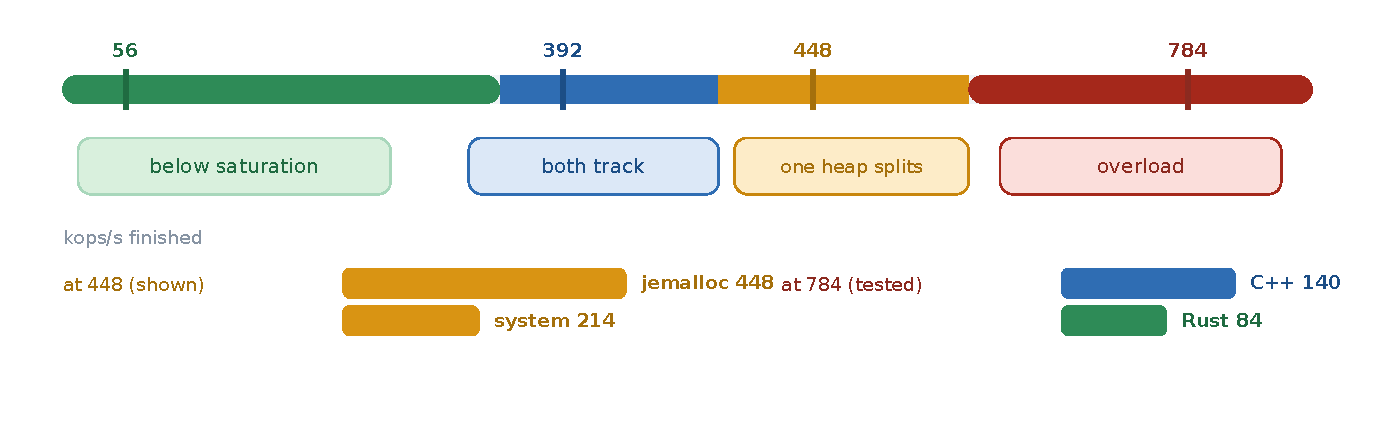
\includegraphics[width=0.78\linewidth]{diagrams/pdf/30_load_regimes.pdf}
\caption[Campaign-clock load regimes on the offered-load axis]{Four operating points on
the offered-load axis, spaced for reading, not to scale. Ticks are
$\ReprLoad$, $\TrackingLoadCpp$, $\TrackingLoadRust$ and
$\OverloadLoad$~kops/s. The comparison at $\KneeGapLoad$ belongs to the
campaign clock and is absent on the later deferred-fill setup. Bars are campaign-clock
throughput there and at
$\OverloadLoad$~kops/s.\label{fig:loadmap}}
\end{figure}

Deeper into overload, at $\OverloadLoad$~kops/s sent, the order flips.
\OverloadSustainedFaster{} still finishes $\OverloadThrCpp$~kops/s where \OverloadSustainedSlower{} finishes $\OverloadThrRust$.
That is a factor of $\OverloadThrRatio$, in \OverloadThrAgree{} runs under both heaps.
The Holm-corrected $p$ is as small as this test family can go, which means the gap is larger than the test can fail to see.
The slower variant uses $\OverloadCpuPerOpRatio$ times the CPU for each call it finishes.
That quantity belongs to the whole campaign process, including the recorder. It does not identify work inside the service.
The bounded queue and the reply handle do not reproduce the order when they are timed alone.

Two later sweeps test the recorder explanation on a separate captured setup.
Each repeats the fourteen-load grid over $\ProbeAfterRuns$ runs, holding the pinned cores, the allocator pair, and the repeat count.
The processor is \ProbeAfterCpu{}, against \MainCpu{} for the campaign.
The later setup has \ProbeAfterNohzFull{} for \texttt{nohz\_full}, against \texttt{\MainNohzFull} in the campaign.
When a sender falls behind, the harness writes up to $\ProbeAfterCap$ extra samples for each finished call.
That extra writing is the fill.
Clock A drops that fill and starts the timer at the actual send.
Its percentiles are coordinated-omission biased on purpose, so its lower Rust p99 is a diagnostic hint. It is not an RQ1 tail result.
Clock B keeps the intended send time and the cap, but writes the fill after the timed window.

Neither diagnostic repeats the large collapse.
With the fill delayed, both languages keep up through $\ProbeAfterTrackRust$~kops/s.
At the top load the system-allocator medians are $\ProbeAfterThrCppSystem$~kops/s for C\texttt{++} and $\ProbeAfterThrRustSystem$ for Rust.
The full \ProbeAfterPairsSystem{} paired repeats cannot tell them apart, at $p = \ProbeAfterThrPSystem$.
Under \texttt{jemalloc}, Rust serves $\ProbeAfterThrRustJemalloc$~kops/s against $\ProbeAfterThrCppJemalloc$ for C\texttt{++}.
The full \ProbeAfterPairsJemalloc{}-pair test resolves that smaller Rust lead at $p \ProbeAfterThrPJemalloc$.
These later $p$-values were computed after seeing the data. They are not adjusted, and they do not join the pre-planned Holm family.
Percentiles on Clock B are the sender falling behind its schedule. They are not the service's own time, so throughput carries this diagnostic.

Clock B also lacks the campaign's uneven knees.
At $\KneeGapLoad$~kops/s the campaign has \KneeGapFaster{} serving $\KneeGapThrFast$~kops/s where \KneeGapSlower{} has fallen to $\KneeGapThrSlow$, a factor of $\KneeGapRatio$.
With the fill delayed, C\texttt{++} serves $\ProbeAfterKneeThrCpp$~kops/s and Rust serves $\ProbeAfterKneeThrRust$.
One gap favoured each language in the campaign. Both disappear on the later setup.
That pattern fits recorder work as the cause.
The host and the kernel setting also changed, so the study cannot claim that the fill timing was the only cause.
The campaign stays the pre-planned comparison.
The later sweeps change how its high-load gaps are read.
They do not give service-latency percentiles after saturation, and they do not establish a general ranking of top rates.
Figure~\ref{fig:overload} compares both clocks at both loads and keeps the two heaps apart.

\begin{figure}[ht]
\centering
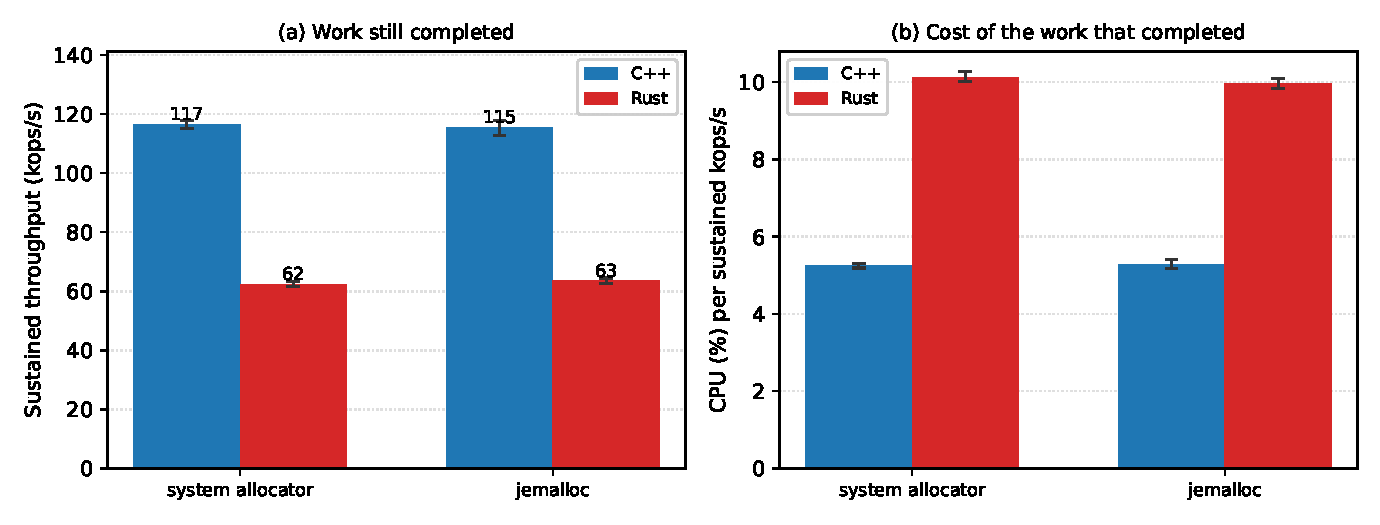
\includegraphics[width=\linewidth]{figures/fig_overload.pdf}
\caption[Campaign and deferred-fill throughput on two captured setups]{Throughput at the
two loads where the campaign shows opposite language gaps. Bars are medians
over \NRepeats{} interleaved repeats with bootstrap $95\%$ intervals. Solid
bars are the \MainCpu{} campaign with \texttt{nohz\_full} on
\texttt{\MainNohzFull}. Hatched bars are the later \ProbeAfterCpu{} diagnostic
with \ProbeAfterNohzFull{} for \texttt{nohz\_full}, where the same fill runs
after the timed window. Panels keep the two heaps separate. The later setup
does not reproduce either large campaign gap.\label{fig:overload}}
\end{figure}

\subsection{Resource use (RQ3)}\label{sec:resources}
The four variants differ in RAM and CPU even where their median delays are close.
Peak resident set size (RSS) is the most memory the process held at once.
On the reported host it contains two effects of similar size.
The Rust build uses $\RssLangDiffLo$--$\RssLangDiffHi$~MiB more peak RAM than the C++ build, under either heap.
Linking \texttt{jemalloc} costs $\RssAllocDiffLo$--$\RssAllocDiffHi$~MiB in either language.
Figure~\ref{fig:resources} shows both effects.
The language effect keeps its direction and its scale in megabytes on all three hosts, but not one exact range.
It spans $\GuestRssLangLo$--$\GuestRssLangHi$~MiB on the guest and $\BmRssLangLo$--$\BmRssLangHi$~MiB on the second bare-metal host.
The allocator effect's size does not travel either.
On the virtual machine it was $\GuestRssAllocOverLang$ times the language effect, $\GuestRssAllocLo$--$\GuestRssAllocHi$~MiB.
Their ratio is therefore a property of the host.
Allocator accounting on the second bare-metal host places the language gap outside the heap.
Rust has $\BmJeMetadataDelta$~MiB more arena metadata, but $\BmJeAllocatedDelta$~MiB less live allocation and $\BmJeResidentDelta$~MiB less allocator-resident memory, while the process peak remains $\BmJeRssDelta$~MiB higher.
The extra RAM is a fixed cost of the process. It is not more live application data.
CPU is a separate result.
At $\ReprLoad$~kops/s Rust uses at most $\CpuDiffAbsMax$ percentage points less.
At $\OverloadLoad$~kops/s the slower campaign-clock variant instead uses $\OverloadCpuPerOpRatio$ times the CPU per finished call.
The deferred-fill sweep does not reproduce that large flip.
That supports a recorder-work explanation, without separating it from the changed setup.
Counters on the second bare-metal host cover only the isolated core call.
Rust retires $\BmInstrDelta\%$ \BmInstrDeltaDir{} instructions and finishes in $\BmCycleDelta\%$ \BmCycleDeltaDir{} cycles, while missing the cache $\BmMissDelta\%$ \BmMissDeltaDir{} often per thousand instructions.
Those counters explain the isolated core result. They do not explain the overload floor.

\begin{figure}[ht]
\centering
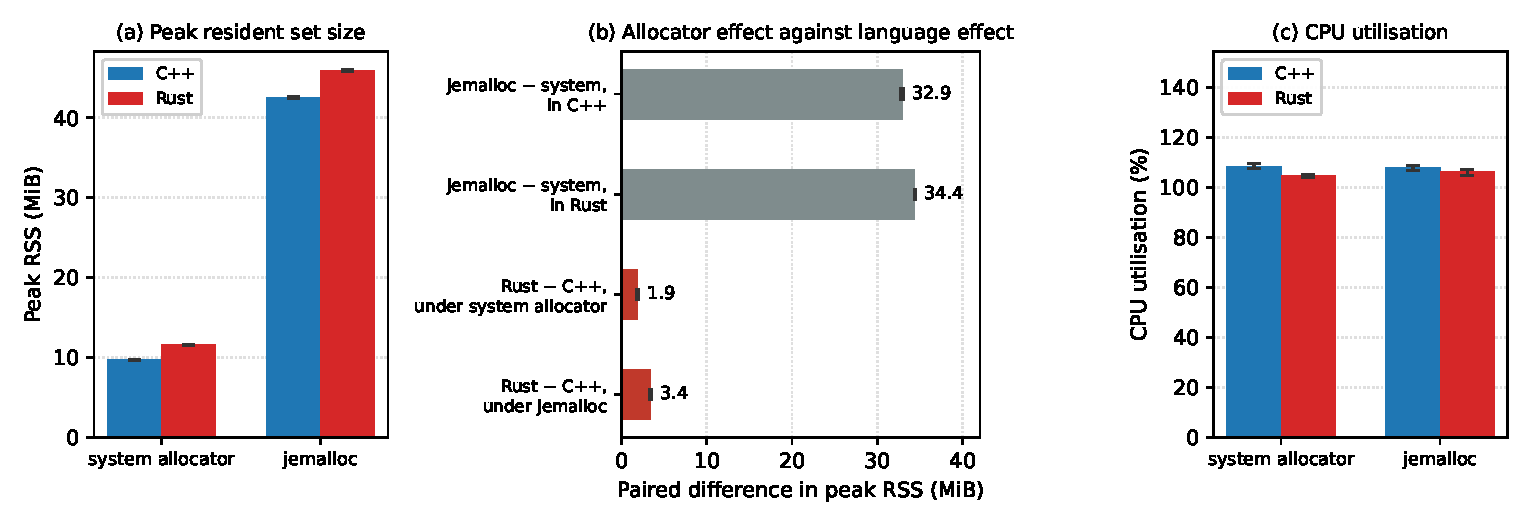
\includegraphics[width=0.78\linewidth]{figures/fig_resources.pdf}
\caption[Resource use, and the two effects inside peak RSS]{Resource use at
$\ReprLoad$~kops/s, grouped by allocator. Bars are medians over \NRepeats{}
repeats with bootstrap $95\%$ intervals, and CPU in (c) is summed across
threads.\label{fig:resources}}
\end{figure}

\subsection{Safety via fault injection (RQ2)}\label{sec:safetyresults}
Safe code is checked by planting $\FaultClasses$ bugs.
Seven come from inside the zone Rust claims to govern.
Seven were chosen because safe Rust is meant \emph{not} to stop them.
Each of the first seven is a compile error in Rust.
In C++ each is valid code.
The bug shows up only if a test drives it, and no single sanitiser hits all seven.
Use-after-move is the case where no sanitiser flags anything.
A moved-from object is still a valid object. Its value is unset.
There is nothing illegal to detect. The name that used to point at the value is simply gone.
All seven boundary cases compile in safe Rust, and then fail when they run.
On two of them the C++ tools are the ones that report the bug.
LeakSanitizer flags the reference cycle that Rust leaks in silence, because leaks are safe in Rust by design~\cite{hughes2025gcrust,cui2024rcanary}.
UndefinedBehaviorSanitizer flags the overflow that Rust defines as wrapping around.
ThreadSanitizer catches the lock-order inversion in $\DeadlockTsanHits$ of $\DeadlockTsanRuns$ runs, a rate that itself jumps around.
It logs lock orders only from locks that return.
If the first inversion waits and never returns, the cycle is never closed, so the tool never flags it.

The seam double-free is the in-guarantee double-free written again through \texttt{unsafe}. It is not a new bug type.
Its C++ half is the same, so only the Rust column moves.
Two Rust model checkers do flag both of the original boundary bugs.
Loom explores thread orders in a way that does not miss a scheduled interleaving.
Shuttle picks orders Loom cannot reach~\cite{bornholt2021shardstore}.
Each bug had to be rewritten in the checker's own parts first, and shrunk to model size.
Miri flags the seam double-free, but it reads Rust and cannot run the C++ host the bug sits behind.
LeakSanitizer and UndefinedBehaviorSanitizer flag without a rewrite.
The two model checkers flag the concurrency boundary cases only after the bug is recast into their parts.
Figure~\ref{fig:taxonomy} draws the whole list as a matrix of outcomes.
Resource Acquisition Is Initialization (RAII) ties cleanup to how long an object lives.
It removes the plain missed unlock, because leaving a scope destroys the guard and releases its lock.
It does not remove the bug type.
Both forgotten-guard programs hang, and neither side's tools said so.

\begin{figure}[ht]
\centering
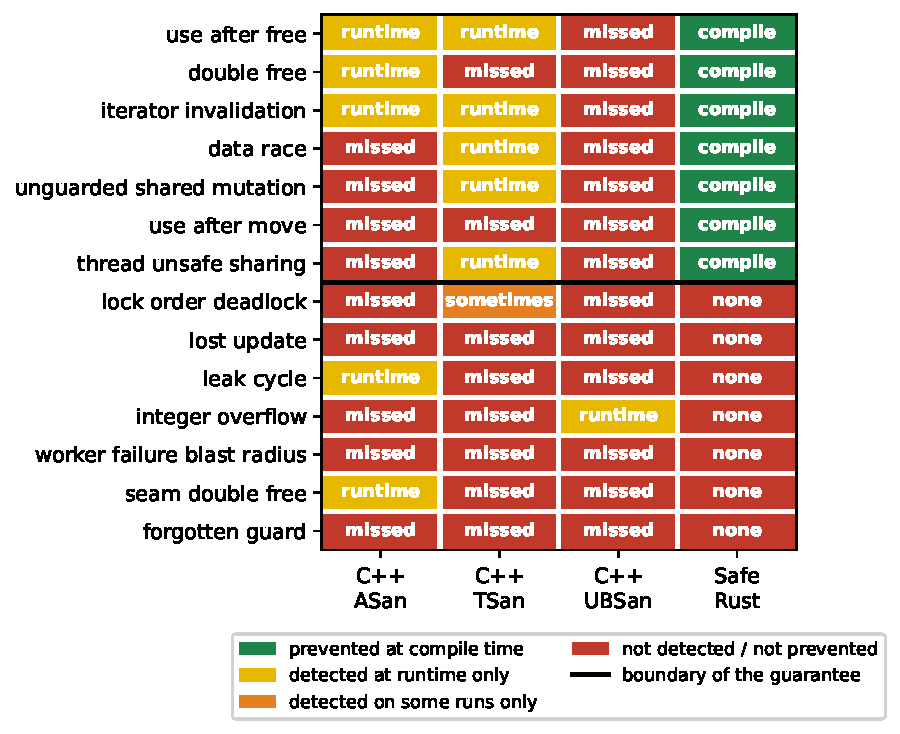
\includegraphics[width=0.72\linewidth]{figures/fig_taxonomy.pdf}
\caption[Where the guarantee stops: the outcome matrix]{The fault-injection
outcomes as a matrix, generated from the taxonomy log.\label{fig:taxonomy}}
\end{figure}

\subsection{Migration (RQ4)}\label{sec:migrationresults}
The FFI seam is the C-ABI layer between the C++ host and the Rust core.
It is small on each measured axis: $\FfiEntryPoints$ C entry points in $\FfiSeamLines$ lines of Rust.
All raw-pointer work is kept in $\FfiUnsafeFns$ functions.
The core is left free of \texttt{unsafe}.
No extra cost is seen against the same signal call made directly.
That bounds any per-call tax at $\FfiOpBoundPct\%$ of that call.
Figure~\ref{fig:ffiseam} shows the structure that bound belongs to.
Three adoption costs beyond the seam were measured as well, and two of them go against the usual worry about taking Rust.
$\BuildDepShareCpu\%$ of the Rust clean build is third-party code.
The project's own source builds in $\BuildAllFirstPartyCpuRatio$ times the CPU time that \texttt{g++} needs.
The $\FootShippedRatio\times$ size gap is a choice of how libraries are linked.
The order flips when that choice is held fixed.
The compared part has no third-party crates and no \texttt{unsafe} sites ($\DepsCore$ crates, $\CoreUnsafe$ \texttt{unsafe} sites).

% After the paragraph the leftover is short of the diagram plus caption, so
% [ht] defers it and \chapter flushes it onto an empty float page. A page
% enlarge plus [!ht] keeps the figure with the subsection that cites it.
\enlargethispage{52pt}
\begin{figure}[!ht]
\centering
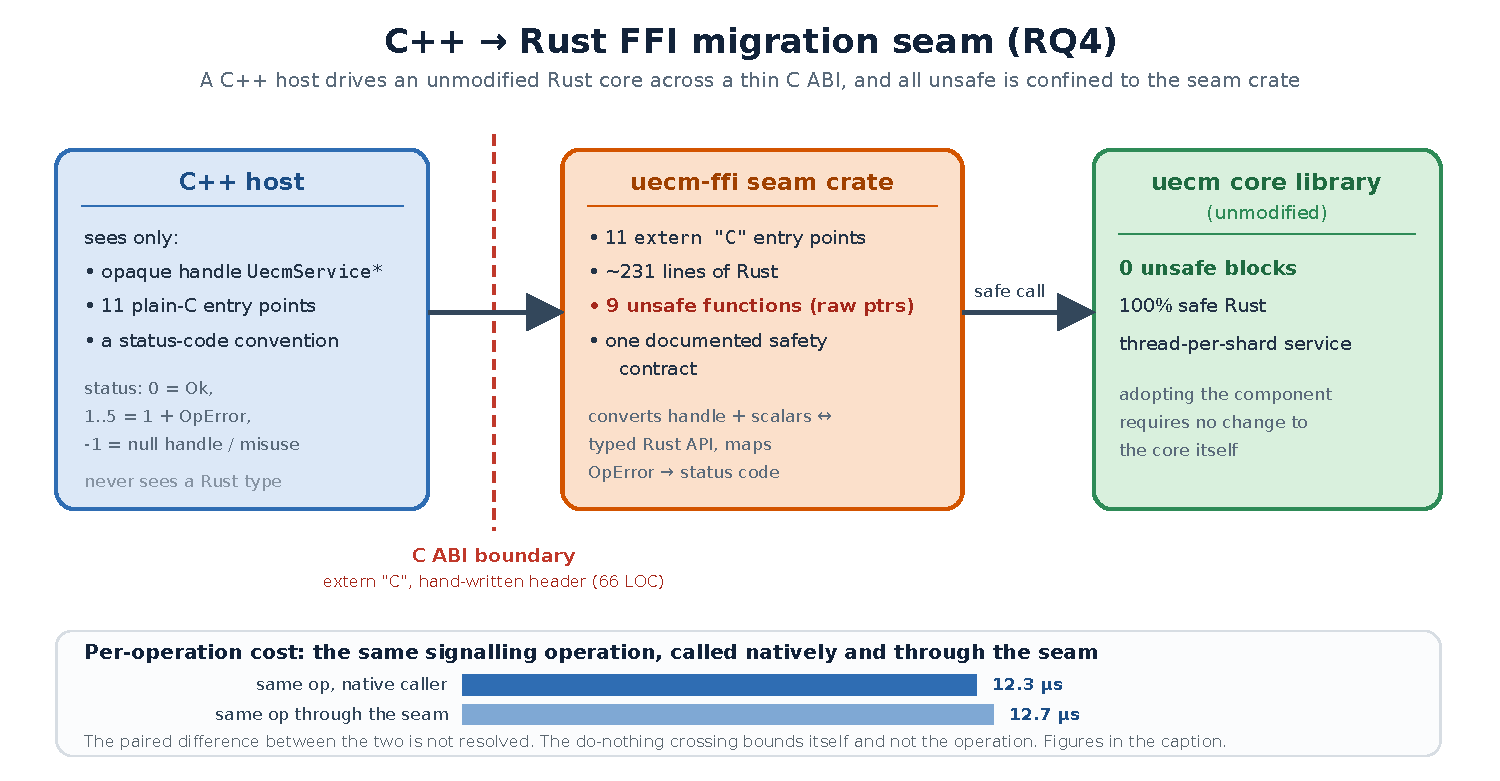
\includegraphics[width=0.78\linewidth]{diagrams/pdf/07_ffi_seam.pdf}
\caption[The C++-to-Rust FFI migration seam]{The C++-to-Rust FFI migration seam.
The same signalling operation costs $\FfiOpNative$~\textmu s directly and
$\FfiOpSeam$~\textmu s through the seam, a paired difference bounded at
$\FfiOpBoundPct\%$ of that call. A do-nothing crossing costs
$\FfiCrossing$~ns and bounds only itself.\label{fig:ffiseam}}
\end{figure}

\chapter{Discussion\label{chapter:discussion}}

\section{Summary of findings}
At $\ReprLoad$~kops/s the variants agree to within $\PFiftyRange\,\mu$s at the median.
The pooled far tail lands on \FarTailLower{}'s side, which means the slowest calls are faster there.
The end-to-end round trip is only $\BudgetCoreShareMax\%$ language work, so it cannot say how large a language effect is.
The same core, timed on its own, is $\BudgetCoreRatio\times$ faster in \BudgetCoreFaster{}.
At higher loads the campaign shows one gap for each language.
Rust leads at $\KneeGapLoad$~kops/s. C++ leads at $\OverloadLoad$~kops/s.
A later captured setup, with the histogram fill delayed, reproduces neither large gap.
That fits recorder work as the cause. It does not separate that cause from the change of machine.
Neither overload clock supplies percentiles of the service's own latency, so RQ1 has no language verdict after saturation.
The RQ2 outcome is complete for the fourteen bug types chosen in advance, and it does not depend on the host.
All seven in-guarantee types are compile errors in safe Rust.
All seven boundary types compile and then fail, in Rust and in C++.
RQ3 finds a higher Rust peak RSS under both heaps: $\RssLangDiffLo$--$\RssLangDiffHi$~MiB on the campaign host, $\GuestRssLangLo$--$\GuestRssLangHi$ on the guest, and $\BmRssLangLo$--$\BmRssLangHi$ on the second bare-metal host.
Below saturation, Rust uses slightly less CPU.
Corrected high-load throughput gives no general language ranking.
RQ4 finds a small seam. Its per-call tax is bounded at $\FfiOpBoundPct\%$ of that call.
API design and learning remain adoption costs that earlier papers describe. This study does not measure their size.

\section{Discussion on the research questions}\label{sec:rqdiscussion}
RQ1 has two answers, split by how hard the service is working.
At $\ReprLoad$~kops/s the campaign resolves differences at the median, at p99, and at p99.9, and the pooled p99.99 lies on Rust's side.
The end-to-end clock still cannot say how large a language effect is, because the core call is only $\BudgetCoreShareMax\%$ of what it times.
After saturation, neither available percentile clock estimates the service's own latency.
The campaign includes fill work on the sender side. Clock B measures the sender falling further behind its schedule.
No ranking of the overload tail follows.

The campaign throughput shows Rust leading at one step and C++ leading later.
The later captured setup reproduces neither large gap when the fill is removed or delayed.
That is evidence for recorder work.
The changed processor and the changed kernel setting stop the study from naming fill timing as the only cause.
Clock A's lower Rust p99 is deliberately biased by coordinated omission. It is not an RQ1 tail result.
Clock B's throughput leaves the system-allocator pair unresolved, and it leaves a smaller Rust lead under \texttt{jemalloc}.
The closest earlier work reports a similar worsening past a threshold rate and attributes it to stackless \texttt{async}/\texttt{await}~\cite{arvidsson2025async}.
That cause cannot apply here, because neither side uses an asynchronous runtime.
Changing Rust's reply handle does not move the floor either.
The campaign ratio is therefore a result about its harness. It does not rank the top rates of the two services.
The prediction written down in advance had named bounds checks and overflow checks as the cause~\cite{zhang2022runtime,harris2023morello}.
That part was wrong.
At normal load the median result still fits evidence that modern out-of-order CPUs absorb most of Rust's safety checks~\cite{balasubramanian2017rust,emmerich2019drivers}.

Some safety bugs are compile errors, so they never become a program that can run.
The seven types Rust does not stop are part of the answer. They were chosen before the runs.
A compiler that will not build a program keeps the bug out of every run.
A sanitiser keeps it out only of the runs a sanitiser test happens to take.
What changes between those two is how much of the running program is covered. The list of bug types stays the same width.
Figure~\ref{fig:boundary} names the mechanism on each side of that line.
Rust reasons about aliasing, which is whether two names refer to the same memory. It does not reason about the order of locks.
A \texttt{Mutex} guard whose lifetime the borrow checker tracks well says nothing about whether two threads take their locks in a matching order.
Static deadlock checks for Rust are an open research problem~\cite{zhang2026deadlock}.
The lost update misses ThreadSanitizer for the same reason it misses the borrow checker.
Where each access is properly synchronised, there is no unsynchronised access to find.
In a field study of $105$ real concurrency bugs, about a third of the cases that were not deadlocks broke the order the writers meant, not their locking~\cite{lu2008mistakes}.
Adopting Rust removes data races. It leaves in place the concurrency bugs that fail quietly.
A migration plan that reads ``memory-safe'' as ``concurrency-safe'' would spend its review effort on the wrong bugs.
In the corpus of Xu et al., every published Rust memory-safety entry in Common Vulnerabilities and Exposures (CVE) involves \texttt{unsafe}, apart from one compiler bug~\cite{xu2021rustcve}.
That is why keeping the core free of \texttt{unsafe} matters.
It is also why \texttt{unsafe} spreading through library crates is a review concern~\cite{evans2020rust}.

\begin{figure}[ht]
\centering
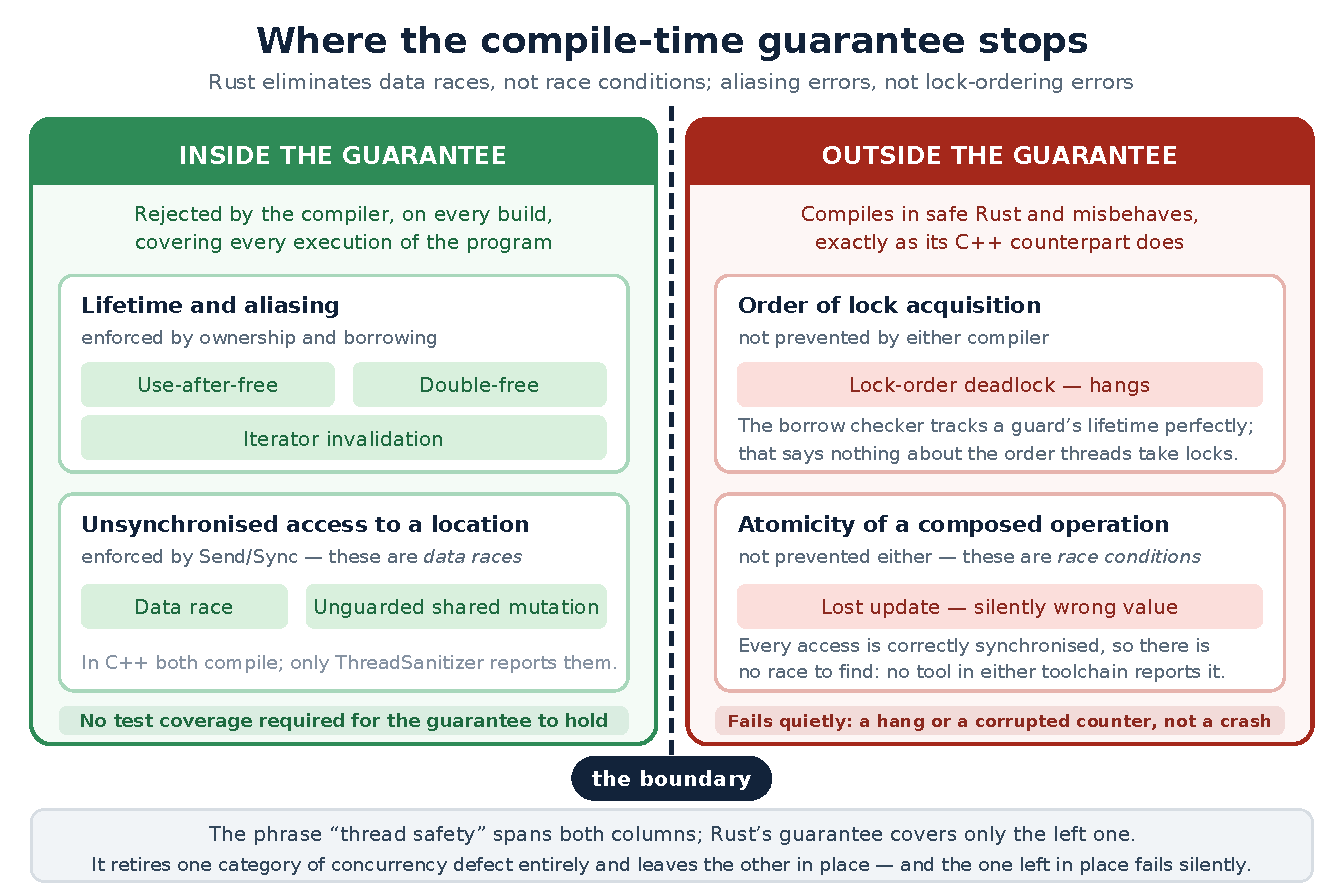
\includegraphics[width=0.78\linewidth]{diagrams/pdf/17_guarantee_boundary.pdf}
\caption[Where Rust's compile-time guarantee stops]{Where Rust's compile-time
guarantee stops, with classes grouped by the mechanism that rejects
them.\label{fig:boundary}}
\end{figure}

One case reaches past the small fault programs.
A gap in the specification let a call be sent outside the window when the service was running.
It passed each test, each parity vector, and all three sanitisers, because nothing ever called that path.
What turned undefined behaviour into a catchable failure on the Rust side was an ordinary bounds check.
It was not a compile-time proof.
The useful thing to plan for is checks that are on by default.
A claim that the compiler has ruled the bug out is stronger than this case supports.
The root cause belongs to the method.
A ban written down with no mechanism behind it leaves each version to fail in its own way.

RQ3 splits by resource, and the splits do not point the same way.
The RAM cost holds under both heaps and on a second host with a new compiler.
Peak RSS is a maximum over the whole run, so the jitter that ruins a p99 does not touch it.
Set beside the heap's own effect, the two are of the same order on both bare-metal hosts.
On the guest the heap's effect was an order of magnitude larger.
The language effect travels from host to host. The ratio of the two effects does not.
The quiet host also places the cost outside the heap, by the heap's own counts.
One close study reports the other direction, with Rust lowest and the gap growing as concurrency rises~\cite{karlback2021ran}.
Those two findings agree once the variants are read as two concurrency runtimes.
Their C++ runs on Boost.Fibers, which gets a stack per fiber.
Their Rust runs on Tokio, where a task is a small future on the heap.
What they timed is the per-task cost of two concurrency runtimes.
Two further studies agree with the direction found here~\cite{olsson2023ranmgmt,sundvisson2026drivers}.
Below saturation, Rust uses slightly less CPU.
The larger flip under the campaign clock is not reproduced with deferred fill, and it cannot be assigned to Rust's safety checks.

RQ4 finds a small seam on the machine side.
A C++ host can call an unchanged Rust core across a thin C-ABI seam.
The cost on a real signal call is bounded at $\FfiOpBoundPct\%$ of that call.
Earlier work names design and learning as human costs~\cite{fulton2021adopting,crichton2024learning}.
This study does not measure their size.
Keeping \texttt{unsafe} at the seam bounds what has to be reviewed. It does not bound what can be corrupted, because the host and the part share one address space~\cite{rivera2021galeed,kirth2022pkrusafe}.
The build time and the binary size point the same way as the seam.
A vendor worried about either should audit its crate budget before blaming the compiler.
The one axis where C++ leads outright is the edit-and-compile loop, for changes that stay inside one source file.
The $\FootShippedRatio\times$ size figure compares two linkage policies. The order flips when the policy is held fixed.

\section{Revisiting the hypotheses}\label{sec:hypotheses}
Section~\ref{sec:rqs} set three hypotheses before any run.
Saying how they came out is what makes this a test.

\begin{description}
  \item[H1] It is not accepted as written.
        No margin for ``close enough'' was defined, so a small but statistically detectable median difference cannot establish that the two languages are equally fast.
        At $\ReprLoad$~kops/s the paired test resolves $\PFiftyDiffAbsMax\,\mu$s, and it resolves differences at the higher percentiles.
        The pooled far tail favours Rust.
        The isolated core favours \BudgetCoreFaster{}.
        After saturation the available clocks do not provide a valid ranking of the service's own latency.
        The hypothesis folded the round trip, the core code, the recorder, and the overload behaviour into one quantity.
        The method cannot support that single quantity.
  \item[H2] For the seven injected types inside the guarantee, it holds with no exception.
        It fails if it is read more loosely than it was written.
        It is accepted for memory safety and for freedom from data races.
        It is rejected for concurrency correctness in general.
        It is a claim about \emph{safe} Rust only.
        The seam case shows the same bug type coming back inside \texttt{unsafe}.
  \item[H3] Any per-call tax is bounded at $\FfiOpBoundPct\%$ of that signalling call.
        The support is the upper bound on the paired difference.
        A difference that fails to reach significance would not, on its own, show that the tax is small.
        The accompanying claim, that the real cost is design and training, is supported by the shape of the result. It is not a statistical test.
\end{description}

\section{Engineering guidelines for incremental adoption}\label{sec:guidelines}
The rules below are the practical form of the findings. Each one carries the limit of the finding behind it.
Choose a first part for how thin its API is. Size is the weaker guide.
Rewriting a rich interface is the schedule risk. The language boundary itself is small.
Keep the C ABI in its own crate, and keep the core free of \texttt{unsafe}.
That keeps \texttt{unsafe} out of the chains of crates it otherwise spreads through~\cite{evans2020rust}.
Leave the concurrency review budget where it is.
Prefer a shared-nothing structure in either language.
The strongest concurrency result here belongs to the design. It belongs to neither compiler.
Plan the learning curve as a training cost, and track it.
Time the inner part as well as the round trip.
Sweep past the point where the service stops keeping up.
Audit every operation on the sender's timed path, including the histogram correction.
Run recorder work after the timed window.
Compare a clock change on the same captured setup before assigning a high-load gap to the service.

\section[Where this study sits]{Where this study sits, and what it cannot support}\label{sec:standing}
The studies closest to this one are the five vendor-hosted theses of Section~\ref{sec:gap}.
Their verdicts clash with each other in every direction.
The one with the opposite sign on peak RAM fits this study once its variants are read as two concurrency runtimes.
Four threats still matter.
The first is that one author wrote both versions.
The same failure mode flipped a printed verdict in this field: the pair looked comparable after a code review, and then Rust was $85$--$91\%$ worse after more speed work~\cite{emberg2023asn1}.
The parity suite bounds what the code does. It does not bound speed.
The second threat is that the end-to-end clock times the design faithfully and the language hardly at all.
Third, the later probes do not share the campaign's processor or its \texttt{nohz\_full} setting.
Their failure to reproduce the two large gaps supports a recorder explanation.
It does not isolate fill timing as the only thing that changed.
No peer-reviewed study reports that same instrument effect.
Fourth, neither high-load clock gives percentiles of the service's own latency.
The campaign includes recorder work. Clock A has coordinated-omission bias. Clock B reports schedule drift.
The thesis therefore leaves the service's latency under overload unresolved.

\section{Ethical and professional reflection}
The study uses no personal data, no subscriber data, and no operator secrets.
All traffic is made for the test.
The service is based on the shape of live code. It is not copied from it, so the artefacts can be shared in public.
The first duty is to avoid claiming too much.
A vendor could read the RQ2 result as permission to describe a moved part as ``safe''.
The boundary cases are why that reading would be wrong.
A deadlocked control plane is an outage.
A lost counter update that stays silent can mislead a mobility decision.
Nothing shown here stops either of those.
The second duty is to say how far the data reaches.
Tail-delay numbers from any single host are a thinner basis for a production roll-out than they look.
That is why the earlier guest sweep is kept.

\chapter{Conclusion and Future Work\label{chapter:conclusions}}

The thesis set modern C++ against Rust.
The object is a UE Context Management service.
It stores the state of each device, as a gNB-CU-CP does.
It looked at four things: how late the slow tail is, which bugs a compile step can stop, what the safety checks cost, and what it costs to add Rust a piece at a time.
Both sides were built from one frozen specification.
They were driven along the same code paths.
That is what lets a language effect be separated from a gap of design or of skill.

The safety mechanisms act at different stages.
Safe Rust rejects all seven injected memory-safety and data-race types before they become programs that can run.
The same seven compile in C++, where a sanitiser can report a bug only if a test executes the relevant path.
All seven boundary types compile and fail in both languages.
On two of them the C++ tools flag a bug that Rust's tools do not.
Rust therefore removes data races and aliasing errors.
It does not remove race conditions, lock-order errors, leaks, wrapping arithmetic, or the blast radius of a failed worker.
It removes nothing inside an \texttt{unsafe} block.
LeakSanitizer and UndefinedBehaviorSanitizer flag two boundary bugs without a rewrite.
The two model checkers flag the concurrency cases only after each bug is recast into their parts.

On migration, the measured seam on the machine side is small.
An unchanged Rust core can be driven from C++ across an FFI seam, the C-ABI layer where the two languages meet.
It has $\FfiEntryPoints$ entry points in $\FfiSeamLines$ lines, and its $\FfiUnsafeFns$ raw-pointer functions contain all of the \texttt{unsafe}.
The core has $\CoreUnsafe$ \texttt{unsafe} sites.
The cost on a real signal call is bounded at $\FfiOpBoundPct\%$ of that call.
Earlier work names API design and the learning curve as adoption costs. This study does not measure their size.
Most of the extra cost of a Rust build is compiling crates, not the compiler's own work on this project.
The size gap is a linkage policy. The order depends on which matched policy is chosen.
Where C++ leads is the edit-and-compile loop, and only for edits that stay inside one source file.

On speed, the data first splits by what is being timed.
The end-to-end clock starts before a sender submits a request and stops after the worker replies.
It includes the queue, the wake-up, and the core call.
Only $\BudgetCoreShareMax\%$ of that round trip is the core work the languages perform, so this clock cannot bound a compiler effect.
A second measurement removes the queue and the cross-thread handoff and times the core call alone.
In that measurement the core is $\BudgetCoreRatio\times$ faster in \BudgetCoreFaster{}.
At the chosen load of $\ReprLoad$~kops/s the paired test finds $\PFiftyDiffAbsMax\,\mu$s in Rust's favour.
At p99.99 the slowest Rust variant sits $\FarTailLangSep\,\mu$s below the fastest C++ one, which means it is that much faster.
The campaign then shows a Rust lead at the knee and a $\OverloadThrRatio\times$ C++ lead deeper into overload.
A later captured setup with deferred fill reproduces neither large gap.
That comparison fits recorder work. The change of setup stops a claim that fill timing was the only cause.
The gaps do not rank the two services, and the service's latency under overload remains unresolved.
On RAM, the Rust build carries a few MiB more of fixed footprint under both heaps.
It does so in the same direction, and on the same megabyte scale, on all three hosts that were timed.
The heap choice costs about as much on both bare-metal hosts, and an order of magnitude more on the guest this study used first.

Taken together, these support a narrow claim.
It applies to stateful, concurrent, partitionable control-plane services of this kind.
Partitionable means the work can be split so that each thread owns its own slice.
At the loads where the service still meets the rate it was sent, the choice is which bug types a team wants to make impossible to write.
The other half of the choice is whether the team will pay the design and training cost of getting there.
Past that load, the campaign includes substantial recorder work and adds no second language ranking.
What the thesis adds is the frozen specification, the pair that passed the same tests, and a timing harness that reaches past saturation.
A split of the round trip says how much of the timed work the language can own.
A bug list maps where the guarantee stops.

Future work answers the gaps one at a time.
The first job is a same-host control that repeats in-run fill and deferred fill on one captured setup.
It would separate recorder timing from the differences in processor and kernel settings.
The next job needs no new host.
It is to vary the transparent hugepage policy on one host, with everything else held fixed.
A hugepage is a larger block of memory than the usual page, and the policy decides when the kernel uses one.
All three hosts agree that the Rust build carries the larger footprint.
They disagree about how that sits against the cost of the heap.
The guest put the heap cost an order of magnitude higher, and neither bare-metal host does.
The hugepage policy is the candidate this study can name but not test, because it was not the same on each host and only the system-allocator variant receives it.
Beyond that, replaying anonymised production traces would check the mix of calls.
The harness can also take further control-plane parts, or the data-heavy layer-2 and physical-layer (PHY) path.
A part with truly shared mutable state would exercise the two sides in a way a shared-nothing design does not.
Testing Rust async runtimes against the thread-per-shard model would separate the runtime from the language in the tail result~\cite{arvidsson2025async}.
Timing what it costs to split the two heaps inside one process would price what it is worth to keep a core free of \texttt{unsafe}~\cite{rivera2021galeed,kirth2022pkrusafe}.
A longer case study would track bug counts and review effort while Rust is added a piece at a time.
That is what would settle the human cost this study can only name.

% Declaration of generative-AI use, required by the University when a language model has
% been used. Shared with Ha_Vien_Mastersthesis_2026.tex: edit ai_statement.tex, not a copy.
%% Declaration of generative-AI use. The University of Helsinki requires a student who
%% has used a language model in preparing a thesis to state in writing which model was
%% used and in what way; the model may not be named as an author or cited as a source.
%%
%% Shared verbatim by Thesis_POC.tex and Thesis_v1.tex so the two cannot drift apart.
%% It uses no generated macros and no chapter numbers, because the two documents number
%% their chapters differently.
%%
%% The order of the paragraphs follows the University's basic reporting instruction:
%% what the use covered, what it was for, which tool, how it performed and how its
%% output was checked, and what the author took from it.

\cleardoublepage
\phantomsection
\addcontentsline{toc}{chapter}{Statement on the Use of AI Tools}
\chapter*{Statement on the Use of AI Tools}
\markboth{Statement on the Use of AI Tools}{Statement on the Use of AI Tools}

\noindent\textbf{Tool.} Anthropic's Claude Opus~5, used through the Cursor development
environment, is the only generative AI system used in the preparation of this thesis. It was
used throughout the work, from June to August~2026. Following University of Helsinki policy the
model is neither named as an author nor cited as a source: it cannot take responsibility for
what it produces, and it cannot reliably vouch for the literature it paraphrases.

\noindent\textbf{What the assistance covered.} It was extensive, and is declared as such. The
model drafted and revised the running prose of this thesis and proposed the order in which its
arguments are made. It wrote and refactored the two implementations of the UE Context
Management service, the load generator, the fault-injection catalogue, and the interoperability
prototype. It wrote the analysis code behind the bootstrap confidence intervals, the exact
paired permutation tests, and the Holm correction, together with the figure-generating and
build scripts and the \LaTeX{} sources. It also suggested candidate literature.
% ==================== ACTION REQUIRED BEFORE SUBMISSION ==========================
% The abstract of Thesis_POC.tex was drafted with model assistance. The University's
% thesis guide states that a language model may not be used when preparing the thesis
% summary, and in this programme the summary also serves as the maturity test, where
% AI use is never permitted. Rewrite the abstract unaided before submitting; until
% that is done the closing sentence of this paragraph is not yet true of Thesis_POC.
% =================================================================================
The abstract was written by the author unaided, as the University's thesis guide requires of
the thesis summary.

\noindent\textbf{What the model did not settle.} The research problem, the four research
questions, and the three hypotheses are the author's, as is the control on which the study's
value rests: freezing one language-neutral specification and one concurrency model, so that the
language remains the only systematic difference between the two implementations. So is the
decision that keeps RQ2 falsifiable, namely to carry two defect classes -- a lock-order deadlock
and a lost update -- that lie outside Rust's compile-time guarantee and can therefore embarrass
the premise rather than confirm it. Every measurement reported here was run by the author on the
hosts documented in this thesis; no measured value came from a language model. Each measured
number reaches the text through a macro regenerated from the raw logs, so a figure cannot be
transcribed by hand, by the author or by the model. The readings of those numbers are the
author's as well, including the two restraints the evidence imposes: that a far tail a
virtualised host cannot resolve must not be reported as equivalence, and that a sweep dominated
by cross-thread handoff cannot bound an effect of the language.

\noindent\textbf{How the output was checked.} Model output was treated as a draft to be
falsified rather than as a result. Claims were checked against the sources cited for them: every
bibliography entry was resolved against Crossref, DataCite, or the issuing body, and each was
traced to the page or clause carrying the claim made of it. That audit found four passages where
the prose overstated or misplaced its source, one of them a sentence inside quotation marks that
does not appear in the work it was attributed to; all four were corrected, and the audit is kept
with the artefacts so that the correction remains reviewable. Code was checked by running it:
the two implementations are held to one conformance suite whose transcripts are diffed line by
line, and the fault catalogue fixes the expected outcome of each defect before it is injected,
so that a surprise appears as a discrepancy instead of being explained away afterwards. Nothing
is asserted here on the model's authority.

\noindent\textbf{What the author took from it.} The model is dependable at mechanical work --
transposing an idiom between two languages, restructuring a table, keeping a build honest -- and
undependable in a specific and predictable way: it will supply a plausible citation for a claim,
a plausible cause for a measurement, and a confident sentence where the data supports a hedge.
Its fluency is not evidence. The lasting lesson of the work was accordingly less about either
language than about verification. The effort saved in drafting is spent again, and rightly, in
checking, and the parts of this thesis that are defensible are the parts that were checked
against a source, a specification, or a measurement.

\noindent\textbf{Responsibility.} The author is responsible for the whole of this thesis: its
language, its facts, its code, its measurements, and its conclusions. Where it is wrong, the
error is the author's.


% STEP 5:
% The bibliography style is selected with the biblatex options in the preamble.

\cleardoublepage %fixes the position of bibliography in bookmarks
\phantomsection

\addcontentsline{toc}{chapter}{\bibname} % This lines adds the bibliography to the ToC
\printbibliography

\end{document}
